\documentclass[a4paper,11pt,openany]{memoir}
\usepackage{amsmath}
%\usepackage[sc,osf]{mathpazo}
%\usepackage[garamond]{mathdesign}
\usepackage{fontspec}
\usepackage[math-style=TeX]{unicode-math}
\usepackage{xunicode}
\usepackage{xltxtra}
\usepackage{polyglossia}
\defaultfontfeatures{Mapping=tex-text}
\setmainfont[   Path=fonts/xits/,
                BoldFont={xits-bold.otf},
                ItalicFont={xits-italic.otf},
                BoldItalicFont={xits-bolditalic.otf},
                SmallCapsFont={../MasticSC-Regular.otf}
            ]{xits-regular.otf}
\setsansfont[   Path=fonts/frutiger/,
                Scale=MatchLowercase,
                BoldFont={FrutigerLTStd-Bold.otf},
                ItalicFont={FrutigerLTStd-Italic.otf},
                BoldItalicFont={FrutigerLTStd-BoldItalic.otf}
            ]{FrutigerLTStd-Roman.otf}
            
\setmathfont{xits-math.otf}
\setmathfont[version=roman,range=\mathcal,Path=fonts/]{latinmodern-math.otf}
%\setmathfont[range=\mathcal,Scale=MatchUppercase]{Lynda Cursive}
%\setmathfont[range=\mathup]{Garamond Premier Pro}
%\setmathfont[range=\mathit]{Garamond Premier Pro}
\setdefaultlanguage{danish}
\setotherlanguage[variant=british]{english}

\usepackage[usenames,dvipsnames,svgnames,table]{xcolor}
\usepackage{graphicx,epic,eepic}
\usepackage{tkz-graph,tkz-euclide}
\usetikzlibrary{calc,intersections,shapes.geometric,decorations.pathmorphing}
\usetikzlibrary{snakes,patterns,plotmarks,decorations.text}
\renewcommand*{\VertexSmallMinSize}{4pt}
\usepackage{tabulary}
\usepackage{pdfpages}
\usepackage{wrapfig}
\usepackage{pifont}
\usepackage{multirow}
\usepackage{colortbl}
\usepackage[normalem]{ulem}

%\renewcommand{\thefootnote}{\fnsymbol{footnote}}

\renewcommand\bibname{References}
\renewcommand{\(}{\begin{equation}}
\renewcommand{\)}{\end{equation}}
\newcommand{\vet}[1]{\underline{#1}}
\newcommand{\mtx}[1]{\underline{\underline{#1}}}
\newcommand{\ono}[1]{\frac{1}{#1}}
\newcommand{\half}{\frac{1}{2}}
\newcommand{\thehead}{}
\newcommand{\head}[1]{\renewcommand{\thehead}{#1}}
\newcommand{\theohead}{}
\newcommand{\ohead}[1]{\renewcommand{\theohead}{#1}}
\newcommand{\thetnote}{}
\newcommand{\tnote}[1]{\renewcommand{\thetnote}{#1}}
\newcommand{\bra}[1]{\left\langle #1 \right|}
\newcommand{\ket}[1]{\left| #1 \right\rangle}
\newcommand{\braket}[2]{\left\langle#1\middle|#2\right\rangle}
\newcommand{\obraket}[3]{\left\langle#1\middle|#2\middle|#3\right\rangle}
\newcommand{\emf}{\mathcal{E}}
\newcommand{\di}{\text{d}}
\newcommand{\atlas}{\textsc{atlas}}
\newcommand{\Atlas}{\textsc{Atlas}}
\newcommand\numberthis{\stepcounter{equation}\tag{\theequation}}

\newenvironment{infilsf}{
    \begin{sffamily}
    \setmathfont[range=\mathup/{num},
                 Scale=MatchLowercase,
                 Path=fonts/frutiger/,
                 ]{FrutigerLTStd-Roman.otf}
    \setmathfont[range=\mathit/{latin,Latin},
                 Scale=MatchLowercase,
                 Path=fonts/frutiger/,
                    ]{FrutigerLTStd-Italic.otf}
    \setmathfont[range=\mathit/{greek,Greek},
                 Scale=MatchLowercase,
                 Path=fonts/dejavu/,
                    ]{DejaVuSans-Oblique.ttf}
    \setmathfont[range=\mathup/{greek,Greek},
                 Scale=MatchLowercase,
                 Path=fonts/dejavu/,
                    ]{DejaVuSans.ttf}
%    \setmathfont[range=\text,
%                 Scale=MatchLowercase,
%                 Path=fonts/frutiger/,
%                    ]{FrutigerLTStd-Roman.otf}
}{
    \setmathfont{xits-math.otf}
    \setmathfont[range=\mathcal,Path=fonts/]{latinmodern-math.otf}
    \end{sffamily}
}

\newenvironment{new}{\color{Blue}}{}

\definecolor{kugray}{RGB}{102,102,102}
\definecolor{kugray1}{RGB}{52,52,52}
\definecolor{natgreen}{RGB}{70,116,60}
\definecolor{natgreen1}{HTML}{63875B}
\definecolor{natgreen2}{HTML}{859B81}
\definecolor{natcomp}{RGB}{134,69,76}
\definecolor{natcomp1}{HTML}{9D696E}
\definecolor{natcomp2}{HTML}{B39598}
\definecolor{natlcomp}{HTML}{5d323d}
\definecolor{natrcomp}{HTML}{52325d}
\definecolor{natyellow}{HTML}{8B6448}
\definecolor{natblue}{HTML}{524F81}
\definecolor{natscatb}{HTML}{3B8178}
\definecolor{natscatg}{HTML}{418B5C}
\definecolor{natscaty}{HTML}{7C8B41}
\definecolor{natscatr}{HTML}{81783C}

\makepagestyle{fancy}

\makepsmarks{fancy}{%
\nouppercaseheads
\createmark{chapter}{left}{nonumber}{}{}
\createmark{section}{right}{shownumber}{}{ \space}
\createplainmark{toc}{both}{\contentsname}
\createplainmark{lof}{both}{\listfigurename}
\createplainmark{lot}{both}{\listtablename}
\createplainmark{bib}{both}{\bibname}
\createplainmark{index}{both}{\indexname}
\createplainmark{glossary}{both}{\glossaryname}}

\makeoddhead{fancy}
   {}{}{}
\makeoddfoot{fancy}{\makebox[0pt][r]{\raisebox{15pt}[20pt]{\textcolor{natgreen}{\rule{1.1\spinemargin}{1pt}}}\makebox[0pt][l]{\raisebox{15pt}[20pt]{\textcolor{natgreen}{\rule{\paperwidth}{1pt}}}}}\textcolor{kugray}{\textsf{\rightmark}}}{}{\textcolor{kugray}{\textsf{\thepage}}}
\makeevenfoot{fancy}{\textcolor{kugray}{\textsf{\thepage}}}{}{\textcolor{kugray}{\textsf{\leftmark}}\makebox[0pt][l]{\raisebox{15pt}{\textcolor{natgreen}{\rule{1.1\spinemargin}{1pt}}}}\makebox[0pt][r]{\raisebox{15pt}{\textcolor{natgreen}{\rule{\paperwidth}{1pt}}}}}
\setlength{\footskip}{40pt}
\pagestyle{fancy}
\aliaspagestyle{chapter}{fancy}

\captionnamefont{\sffamily\color{natgreen}\bfseries} \captiontitlefont{\footnotesize} \captionstyle{\\}
\renewcommand*{\printchaptername}{}
\renewcommand*{\chapternamenum}{}
\renewcommand*{\afterchapternum}{}
\renewcommand{\chapnumfont}{\chaptitlefont\sffamily\HUGE}
\renewcommand{\printchapternum}{\chapnumfont \colorbox{natgreen}{\textcolor{white}{\hspace{.2em}\thechapter\hspace{.2em}}}\hspace{1em}}
\setsecheadstyle{\large\bfseries}
\setsubsecheadstyle{\bfseries}
\setsubsubsecheadstyle{}
\setsecnumformat{\textsf{\color{natgreen}\csname the#1\endcsname\quad}}
\maxsecnumdepth{subsubsection}
\renewcommand{\labelenumi}{\sffamily\bfseries\color{natgreen}\theenumi.}
\renewcommand{\labelitemi}{\color{natgreen}\ding{110}}
\renewcommand{\labelitemii}{\color{natgreen}\textbullet}
\setcounter{tocdepth}{2}

\setlength{\arrayrulewidth}{2pt}

\newsubfloat{figure}

\begin{hyphenrules}{danish}
\hyphenation{be-stem-mes}
\hyphenation{rest-klas-se-sæt-ning}
\end{hyphenrules}
\begin{hyphenrules}{english}
\hyphenation{Ham-il-ton}
\hyphenation{ATLAS}
\hyphenation{Atlas}
\hyphenation{atlas}
\hyphenation{CERN}
\hyphenation{i-den-ti-cal}
\hyphenation{pro-vid-ed}
\hyphenation{Calc-HEP}
\hyphenation{par-ticles}
\hyphenation{brems-strahl-ung}
\end{hyphenrules}
\usepackage[pdfusetitle]{hyperref}
\urlstyle{sf}

\begin{document}
\begin{english}

\chapter{Theory}
In order to test the Standard Model by observing proton-proton collisions, we must be able to predict the outcome of such collisions using the SM.

As the SM is a quantum field theory, what we can calculate is the probability $\mathcal P$ of going from some initial to some final state, the effect of which is that we only observe that outcome in the detector in a fraction of the events. At a high level, the collision experiment involves shooting things at other things, we can consider this analogous to the case where, out of a number of projectiles fired at some target, only as a fraction actually hit. That fraction that will obviously depend on the cross sectional area of the target. Indeed, the number of hits, $N$, will depend on the number of projectiles $N_P$, the number of targets $N_T$, the cross section $\sigma$ and the size of the area the projectiles can strike within $A$ as
\[N=\frac{N_PN_T\sigma}{A}.\]
From this, we deduce that the probability of a single projectile striking a single target equals $\sigma/A$. In this form, we are still mixing the kinematic probability for two particles coming close enough to interact with the dynamic probability of a particular interaction occurring. We can fix this by expressing the probability $\mathcal P$ as a function of the separation between the interacting particles, given by the impact parameter $\mathbf b$, and then integrating over all $\mathbf b$. Then, we can write
\[\sigma=\int d^2b\,\mathcal P(\mathbf b)\propto\mathcal P(\text{in}\rightarrow\text{out})=\left|\braket{\phi\cdots\phi_\text{out}}{\phi\cdots\phi_\text{in}}\right|^2.\]
In this way, we can calculate the cross section of some process from its transition amplitude.

\section{The Lagrangian formulation of QFT}

In classical mechanics \cite{goldstein}, the Lagrangian formulation describes the path taken by a system between a given initial and final state---a particle with an initial and a final position, say---by finding the path that minimises the action $S$, which is defined as the integral along a given path over the Lagrangian $L$:
\[S[q]=\int_\textrm{path}dtL[q,\dot{q},\ldots],\]
where $q$ is a generalised coordinate. In the picture, the Lagrangian encapsulates the dynamics of the system. It is related to the Hamiltonian $H$ by
\(L = p\dot q- H,\label{htol}\)
where $p$ is momentum.

In quantum mechanics, the probability of going from one state to another is given as the absolute square of the transition amplitude \cite{sred:tramp},
\[\bra{q\prime}e^{-i\hat H(t\prime-t)}\ket{q}\]
where $\hat H$ is the Hamiltonian of the system. This can be written as
\(\int\,\mathcal Dq\,\mathcal Dp\,\exp\left[i\int_t^{t\prime}dt\,[p(t)\dot q(t)-H(p(t),q(t))]\right],\label{e.Dq}\)
where the integral is over all paths with position $q$ at time $t$ and position $q\prime$ at time $t\prime$. We recognise the expression in the innermost integral from eq.~\eqref{htol}. To relate this back to the classical case, we expect the paths close to the classical path to give a large contribution, while paths far from the classical path cancel out.

The Lagrangian has the added feature that, for a local theory, it is possible to write it as a spatial integral over the Lagrangian density:
\[L=\int \,d^3x\,\mathcal L.\]
Thus, the action can be written as
\(S=\int\,d^4x\,\mathcal L,\label{e.S}\)
which is manifestly Lorenz invariant, so long as $\mathcal L$ is a Lorenz scalar. Given the ubiquity of local quantum field theories, it is common in this field to drop `density' from the name, and refer to $\mathcal L$ as the Lagrangian.

With this, we have an expression for the cross section of a transition from one state to another in terms of the Lagrangian $\mathcal L$, which describes a physical model. Let us now use as an example, the simple model described by the following Lagrangian:
\[\mathcal L= \half\partial^\mu\phi\partial_\mu\phi-\half m^2\phi^2-\frac{\lambda}{4!}\phi^4=\phi[\partial^2-m^2]\phi-\frac{\lambda}{4!}\phi^4\]
This is an example of $\phi^4$ theory. From the form of the Lagrangian, we can spot a term that describes a propagator, and one for a four-way interaction. With this, we should be able to evaluate a transition amplitude by simply dropping this expression into eq.~\eqref{e.S} and \eqref{e.Dq} and writing
\[A = \int\mathcal D\phi\,e^{iS[\phi]}.\label{e.Dphi}\]
There is still some work left before this can be evaluated.

Expressing $\phi(x)$ in terms of its Fourier modes,
\[\phi(x)=\int\frac{d^4k}{(2\pi)^4}e^{ikx}\tilde\phi(k)\]
(note that $x$ and $k$ are four-vectors), the Lagrangian becomes
\begin{align*}\mathcal L=&-\int\frac{d^4k}{(2\pi)^4}\frac{d^4k\prime}{(2\pi)^4} e^{i(k+k\prime)x}\tilde\phi(k)[kk\prime +m^2]\tilde\phi(k\prime)\\
&-\frac{\lambda}{4!}\int\frac{d^4k_1\,d^4k_2\,d^4k_3\,d^4k_4}{(2\pi)^{16}}e^{i(k_1+k_2+k_3+k_4)x}\tilde\phi(k_1)\tilde\phi(k_2)\tilde\phi(k_3)\tilde\phi(k_4)
\end{align*}
We find the action of this model by inserting this expression for $\mathcal L$ into eq.~\eqref{e.S}. $x$ only appears as a phase factor, which means that integrating over $x$ only produces delta functions:
\begin{align*}
S=&\int\frac{d^4k}{(2\pi)^4}\tilde\phi(-k)(k^2-m^2)\tilde\phi(k)\\
&-\frac{\lambda}{4!}\int\frac{dk_1\,dk_2\,dk_3\,dk_4}{(2\pi)^3}\tilde\phi(k_1)\tilde\phi(k_2)\tilde\phi(k_3)\tilde\phi(k_4)\delta(k_1+k_2+k_3+k_4),
\end{align*}
where we used the delta-function in the first term to identify $k\prime=-k$. The first term of the action describes the free part of the theory, and the second term describes the interacting part, so we will call them $S_F$ and $S_I$, respectively. Working from this expression for $S$, we can Taylor expand the integrand in $\lambda$:
\[e^{iS}=e^{i(S_F+S_I)}=e^{iS_F}\left(1-iS_I+\frac{(-iS_I)^2}{2}+\frac{(-iS_I)^3}{3!}+\frac{(-iS_I)^4}{4!}+\cdots\right)\]
This assumes that $\lambda$ is sufficiently small, making the interaction term a small pertubation of the theory. Assuming this to be the case, the interacting theory is expressed as a series of corrections to the free theory.

Given a state $\ket{\phi_k}$, which represents a particle with a definite four--momentum $k$, we can write
\[\ket{\phi_k}=\int\frac{d^4k}{(2\pi)^4}\tilde\phi(k)\ket{k}.\]
The transition amplitude for going from one such state to another can then be written, via eq.~\eqref{e.Dq}, as
\[\braket{\phi_1}{\phi_A}=\int\mathcal D\phi\frac{d^4k_1}{(2\pi)^4}\frac{d^4k_A}{(2\pi)^4}\,\phi(k_1)\phi(k_A)e^{iS[\phi]}.\]
Leaving the momentum integrals aside for the moment, and suppressing some factors of $2\pi$, which will eventually cancel out, the first term in the expansion of $e^{iS}$ gives the expression
\[\int\mathcal D\phi\,\phi(k_1)\phi(k_A)e^{iS_F},\]
which is a Gaussian integral. Assuming the participating momenta are identical, it has the solution \cite{griffiths:gauss}
\[\frac{\delta^4(k_A-k_1)}{k^2-m^2}\int\mathcal D\phi\,e^{iS_F},\] 
where the delta function has been introduced to ensure that $k_A=k_1$, meaning that momentum conservation is imposed. The remaining integral is a constant independent of $\phi$, which is absorbed in the normalisation. The remaining expression is the propagator in momentum space. 
 
When we return to carrying out the $k$ integrals, we will find that there is a singularity at $k^2=m^2$, which can be avoided by slightly modifying the integration path. Feynman's prescription for modifying the path yields the expression $(k^2-m^2+i\epsilon)^{-1}$, the Feynman propagator in momentum space. 

The second term in the expansion of $e^{iS}$ yields\footnote{Here, $\phi^n$ is shorthand for a product of $n$ $\tilde\phi$ functions of seperate momenta.} 
\[-\frac{i\lambda}{4!}\delta^4(p_1+p_2+p_3+p_4)\int\mathcal D\phi\,\phi^6e^{iS_F}.\] 
Solving the Gaussian integral gives a sum of terms of the form 
\(-\frac{i\lambda}{4!}\delta^4(p_1+p_2+p_3+p_4)\frac{\delta^4(k_1-p_1)}{{k_1}^2-m^2}\frac{\delta^4(p_2-p_3)}{{p_2}^2-m^2}\frac{\delta^4(p_4-k_A)}{{k_A}^2-m^2},\label{1t1f}\)
where the momenta are paired in all possible combinations. There are $6!$ different combinations, but they fall into only two topoligically inequivalent groups, as illustrated in figure~\ref{fey1t1o2}.

\begin{figure}[htb]
\begin{minipage}{.65\textwidth}
\begin{footnotesize}\begin{center}
\begin{tikzpicture}
\draw (-3,0) node[left]{$1$} -- 
      ++(1,.5) to[in=45,out=135,min distance=15mm,looseness=8] ++(0,0) --
      ++(1,-.5) node[right]{$A$};
\draw (1,.2) node[left]{$1$} -- ++(2,0) node[right]{$A$} 
      ++(-1,.5) to[in=45,out=-45,min distance=15mm,looseness=8] 
      ++(0,0) to[in=225,out=135,min distance=15mm,looseness=8] ++(0,0);
\end{tikzpicture}
\end{center}\end{footnotesize}
\end{minipage}
\hfill
\begin{minipage}{.3\textwidth}
\begin{center}\begin{footnotesize}
\begin{tikzpicture}
\draw (-1,0) node[left]{$1$} -- (1,0) node[right]{$A$};
\end{tikzpicture}
\end{footnotesize}\end{center}
\end{minipage}
\begin{minipage}[t]{.65\textwidth}
\caption{The two structurally distinct groups of terms in the solution of the second term in the expansion of $e^{iS}$ for the $1\rightarrow1$ transition amplitude, illustrated by drawing the propagators as lines between either the in- and outgoing states $A$ and $1$ or a vertex connecting four lines, which represents the delta function of $p$-momenta.  There are $4!$ different ways to combine the ingoing lines, which means each interaction gets a symmetry factor of $4!$, which is neatly cancelled by the factor of $(4!)^{-1}$ in the original term.
\label{fey1t1o2}}
\end{minipage}
\hfill
\begin{minipage}[t]{.3\textwidth}
\caption{The first term drawn with the same method as fig.~\ref{fey1t1o2}.\label{fey1t1o1}}
\end{minipage}
\end{figure}

Using the same method to illustrate the first term in the expansion gives the somewhat less interesting one shown in fig.~\ref{fey1t1o1}.

\begin{figure}[htb]
\hfill
\begin{tikzpicture}
\draw (-3,1) -- (-1,-1) (-3,-1) -- (-1,1);
\node[right] at (-1,0) {$=-i\lambda$};
\end{tikzpicture}
\hfill
\begin{tikzpicture}
\node[right] at (-1,0) {$=\dfrac{1}{k^2-m^2}$};
\draw (-3,0) -- (-1,0);
\node at (0,-1) {};
\node at (0,1) {};
\end{tikzpicture}
\hfill \phantom{d}
\caption{The building blocks for Feynman diagrams in $\phi^4$ theory. Once constructed, find the momentum of each propagator by imposing momentum conservation at each vertex. Any momentum that cannot be related to one of the external momenta is integrated over.
\label{phi4rules}}
\end{figure}

\underline{These are Feynman diagrams, and, using the Feynman rules laid out in figure~\ref{phi4rules}, the procedure can be reversed, so that first all those topologically inequivalent diagrams that have the right external connections are constructed using the components allowed by the Feynman rules, and then the value given to each such diagram is found, possibly multiplied by an symmerty factor, and used in later calculations.}

Looking at eq.~\eqref{1t1f}, one of the internal $p$ momenta can not be fixed to the external $k$ momenta, which leaves this term proportional to a diverging integral, associated with the looping line in the left diagram in fig.~\ref{fey1t1o2}. There are established methods for renormalising these divergent terms, however for the present purposes, we note simply that non-divergent terms result from the lowest orders in the expansion, and become more common at higher orders, terms can alternatively be ordered by the number of loops in their diagrams. The non-divergent terms with loopless diagrams are referred to in the scheme as leading order (LO) terms, terms with single-loop diagrams are called next-to leading order (NLO), and so on.

\section{Feynman diagrams}\footnote{The derivation in this section is inspired by \cite{wiki.feydiag}}

Attempting this method in the case of a two particle state going to another two particle state, we can construct to zeroth order in $\lambda$, the Feynman diagrams in figure~\ref{efeydig1}.
\begin{figure}[hbt]
\begin{footnotesize}\begin{center}
\begin{tikzpicture}
\draw (-4,1) node[left]{$1$} -- (-2,1) node[right]{$A$};
\draw (-4,-1) node[left]{$2$} -- (-2,-1) node[right]{$B$};
\draw (0,0) node{{\normalsize $+$}};
\draw (2,1) node[left]{$1$} -- (4,-1) node[right]{$B$};
\draw[line width=5pt,white] (2,-1) -- (4,1) ;
\draw (2,-1) node[left]{$2$} -- (4,1) node[right]{$A$};
\end{tikzpicture}
\end{center}\end{footnotesize}
\caption{The Feynman diagrams associated with the first term in the expansion of the $2\rightarrow2$ transition amplitude. Once again, connected states are required to have the same momentum, however with more particles going into and coming out of the process, there are more than one way of connecting the ingoing and outgoing states.
\label{efeydig1}}
\end{figure}

The value of these diagrams, using the rules, is
\[\frac{\delta^4(k_1-k_A)}{{k_1}^2-m^2}\frac{\delta^4(k_2-k_B)}{{k_2}^2-m^2}+\frac{\delta^4(k_1-k_B)}{{k_1}^2-m^2}\frac{\delta^4(k_2-k_A)}{{k_2}^2-m^2},\]
which is indeed what we would get from solving the Gaussian integral, up to some symmetry factors. At the next order in $\lambda$, we can build the diagrams in fig.~\ref{efeydig2}.

\begin{figure}[hbt]
\begin{footnotesize}\begin{center}
\begin{tikzpicture}[scale=.75]
\draw (-6.5,0) to [in=225,out=315,min distance=25mm,looseness=8] (-6.5,0) to [in=135,out=45,min distance=25mm,looseness=8] (-6.5,0);
\draw (-5,0) node{\normalsize$\times$};
\draw (-4,0) node{$\left(\text{\tikz[scale=.75] \draw (0,1) (0,-1);}\right.$};
\draw (-3,1) node[left]{$1$} -- (-1,1) node[right]{$A$};
\draw (-3,-1) node[left]{$2$} -- (-1,-1) node[right]{$B$};
\draw (0,0) node{{\normalsize $+$}};
\draw (1,1) node[left]{$1$} -- (3,-1) node[right]{$B$};
\draw[line width=5pt,white] (1,-1) -- (3,1) ;
\draw (1,-1) node[left]{$2$} -- (3,1) node[right]{$A$};
\draw (4,0) node{$\left)\text{\tikz[scale=.75] \draw (0,1) (0,-1);}\right.$};
\draw (5.5,0);
\end{tikzpicture}

\vspace{.5em}

\begin{tikzpicture}[scale=.75]
\draw (1,1) node[left]{$1$} -- ++(2,0) node[right]{$A$}
      ++(-2,-2) node[left]{$2$} -- 
      ++(1,0) to[in=45,out=135,min distance=15mm,looseness=8] ++(0,0) --
      ++(1,0) node[right]{$B$};
\draw (4,0) node{\normalsize $+$};
\draw (5,1) node[left]{$1$} -- 
      ++(1,0) to[in=225,out=315,min distance=15mm,looseness=8] ++(0,0) --
      ++(1,0) node[right]{$A$}
      ++(-2,-2) node[left]{$2$} -- 
      ++(2,0) node[right]{$B$};
\draw (8,0) node{\normalsize $+$};
\draw (9,1) node(p1)[left]{$1$} -- ++(2,-2) node[right]{$B$};
\draw[line width=5pt,white] (p1.east) ++(0,-2) -- ++(2,2);
\draw (p1.east) ++(0,-2) node[left]{$2$} --
      +(.5,.5) to[in=180,out=90,min distance=15mm,looseness=8] +(0.5,0.5) --
      ++(1.5,1.5) node[right]{$A$};
\draw (12,0) node{\normalsize $+$};
\draw (13,1) node(p2)[left]{$1$} -- 
      +(.5,-.5) to[in=180,out=270,min distance=15mm,looseness=8] +(0.5,-0.5) --
      ++(1.5,-1.5) node[right]{$B$};
\draw[line width=5pt,white] (p2.east) ++(0,-2) -- ++(2,2);
\draw (p2.east) ++(0,-2) node[left]{$2$} --
      ++(2,2) node[right]{$A$};
\end{tikzpicture}

\vspace{.5em}

\begin{tikzpicture}[scale=.75]
\draw (1,1) node[left]{$1$} -- (3,-1) node[right]{$B$};
\draw (1,-1) node[left]{$2$} -- (3,1) node[right]{$A$};
\end{tikzpicture}

\end{center}\end{footnotesize}
\caption{The Feynman diagrams associated with the second term in the expansion of the $2\rightarrow2$ transition amplitude. The joining of four momemta by the last delta function is illustrated by having four lines meet in a point.
\label{efeydig2}}
\end{figure}

Of these diagrams, those in the first two lines are simply those of fig.~\ref{efeydig1} with loops added, and can be considered the one-loop, or next-to leading order, part of those processes. The only new diagram is the one in the last line, which describes an interaction between the two ingoing fields.

The full development of all this into the Standard Model and its underlying framework, which has only been outlined here, is the subject of any number of texts (eg. \cite{srednicki}), and will not be given any further treatment here. The upshot is that the SM contribution to the $q\bar q\rightarrow\gamma\gamma$ process can now be summarised in a single, though admittedly bipartite, figure, namely fig.~\ref{smfeyn}, at least to next-to leading order.

\begin{figure}[htb]
\parbox[t]{.45\textwidth}{\begin{center}\begin{footnotesize}\begin{tikzpicture} [>=triangle 45]
\draw[>-] (-1,1) -- (0,1);
\draw[->] (0,1) -- (0,0);
\draw[<-] (-1,-1) -- (0,-1) -- (0,0);
\draw (-2,1) node[left] {$q$} -- (-1,1);
\draw (-2,-1)  node[left] {$\bar q$} -- (-1,-1);
\draw[snake=coil,segment aspect=0] (0,1) -- (2,1) node[right] {$\gamma$};
\draw[snake=coil,segment aspect=0] (0,-1) -- (2,-1) node[right] {$\gamma$}; 
\end{tikzpicture}
\end{footnotesize}\end{center}
\subcaption{SM contribution at tree level. \label{lofeyn}}}\hfill
\parbox[t]{.52\textwidth}{\begin{center}\begin{footnotesize}
\begin{tikzpicture} [>=triangle 45]
\draw[>-] (-1,1) -- (0,1);
\draw[decorate, decoration={coil,amplitude=2pt, segment length=2.68pt}] 
    (0,1) -- node[below]{$g$} (2,1) ;
\draw[decorate, decoration={coil,amplitude=2pt, segment length=2.68pt}] 
    (2,1) -- node[left]{$g$} (2,-1);
\draw[decorate, decoration={coil,amplitude=2pt, segment length=2.68pt}] 
    (2,-1) -- node[above]{$g$} (0,-1); 
\draw[decorate, decoration={coil,amplitude=2pt, segment length=2.68pt}] 
    (0,-1) -- node[right]{$g$} (0,1);
\draw[<-] (-1,-1) -- (0,-1);
\draw (-2,1) node[left] {$q$} -- (-1,1);
\draw (-2,-1)  node[left] {$\bar q$} -- (-1,-1);
\draw[decorate, decoration={snake}] (2,1) -- (4,1) node[right]{$\gamma$};
\draw[decorate, decoration={snake}] (2,-1) -- (4,-1) node[right]{$\gamma$};
\end{tikzpicture}
\end{footnotesize}\end{center}
\subcaption{SM contribution at loop level. $g$s mark gluons.}}\hfill
\caption{Feynman diagrams of the Standard Model contributions to the $q\bar q\rightarrow\gamma\gamma$ process up to next to leading order.\label{smfeyn}}
\end{figure}


We can calculate the invariant mass of a photon pair, defined as \cite{marshaw:invmass}
\begin{align*} 
M_{\gamma\gamma}&=\sqrt{(E_1+E_2)^2+|\mathbf p_1+\mathbf p_2|^2},
\intertext{which, in the case of massless particles, can be rewritten as}
&=\sqrt{2p_1p_2(1-\cos\theta)}. \label{sinvmass}
\end{align*}
The distribution of invariant mass for diphoton events can be used to characterise the underlying processes. Before any modifications to the SM are introduced, the distribution of invariant masses can be examined by producing a number of simulated pseudo-experiments, in this case using the event generator CalcHEP \cite{calchep}. The distribution is displayed in fig.~\ref{sminvm}.

\begin{figure}[hbt]
\begin{minipage}[b]{.69\textwidth}

\begin{sffamily}

\pgfdeclareplotmark{cross} {
\pgfpathmoveto{\pgfpoint{-0.3\pgfplotmarksize}{\pgfplotmarksize}}
\pgfpathlineto{\pgfpoint{+0.3\pgfplotmarksize}{\pgfplotmarksize}}
\pgfpathlineto{\pgfpoint{+0.3\pgfplotmarksize}{0.3\pgfplotmarksize}}
\pgfpathlineto{\pgfpoint{+1\pgfplotmarksize}{0.3\pgfplotmarksize}}
\pgfpathlineto{\pgfpoint{+1\pgfplotmarksize}{-0.3\pgfplotmarksize}}
\pgfpathlineto{\pgfpoint{+0.3\pgfplotmarksize}{-0.3\pgfplotmarksize}}
\pgfpathlineto{\pgfpoint{+0.3\pgfplotmarksize}{-1.\pgfplotmarksize}}
\pgfpathlineto{\pgfpoint{-0.3\pgfplotmarksize}{-1.\pgfplotmarksize}}
\pgfpathlineto{\pgfpoint{-0.3\pgfplotmarksize}{-0.3\pgfplotmarksize}}
\pgfpathlineto{\pgfpoint{-1.\pgfplotmarksize}{-0.3\pgfplotmarksize}}
\pgfpathlineto{\pgfpoint{-1.\pgfplotmarksize}{0.3\pgfplotmarksize}}
\pgfpathlineto{\pgfpoint{-0.3\pgfplotmarksize}{0.3\pgfplotmarksize}}
\pgfpathclose
\pgfusepathqstroke
}
\pgfdeclareplotmark{cross*} {
\pgfpathmoveto{\pgfpoint{-0.3\pgfplotmarksize}{\pgfplotmarksize}}
\pgfpathlineto{\pgfpoint{+0.3\pgfplotmarksize}{\pgfplotmarksize}}
\pgfpathlineto{\pgfpoint{+0.3\pgfplotmarksize}{0.3\pgfplotmarksize}}
\pgfpathlineto{\pgfpoint{+1\pgfplotmarksize}{0.3\pgfplotmarksize}}
\pgfpathlineto{\pgfpoint{+1\pgfplotmarksize}{-0.3\pgfplotmarksize}}
\pgfpathlineto{\pgfpoint{+0.3\pgfplotmarksize}{-0.3\pgfplotmarksize}}
\pgfpathlineto{\pgfpoint{+0.3\pgfplotmarksize}{-1.\pgfplotmarksize}}
\pgfpathlineto{\pgfpoint{-0.3\pgfplotmarksize}{-1.\pgfplotmarksize}}
\pgfpathlineto{\pgfpoint{-0.3\pgfplotmarksize}{-0.3\pgfplotmarksize}}
\pgfpathlineto{\pgfpoint{-1.\pgfplotmarksize}{-0.3\pgfplotmarksize}}
\pgfpathlineto{\pgfpoint{-1.\pgfplotmarksize}{0.3\pgfplotmarksize}}
\pgfpathlineto{\pgfpoint{-0.3\pgfplotmarksize}{0.3\pgfplotmarksize}}
\pgfpathclose
\pgfusepathqfillstroke
}
\pgfdeclareplotmark{newstar} {
\pgfpathmoveto{\pgfqpoint{0pt}{\pgfplotmarksize}}
\pgfpathlineto{\pgfqpointpolar{44}{0.5\pgfplotmarksize}}
\pgfpathlineto{\pgfqpointpolar{18}{\pgfplotmarksize}}
\pgfpathlineto{\pgfqpointpolar{-20}{0.5\pgfplotmarksize}}
\pgfpathlineto{\pgfqpointpolar{-54}{\pgfplotmarksize}}
\pgfpathlineto{\pgfqpointpolar{-90}{0.5\pgfplotmarksize}}
\pgfpathlineto{\pgfqpointpolar{234}{\pgfplotmarksize}}
\pgfpathlineto{\pgfqpointpolar{198}{0.5\pgfplotmarksize}}
\pgfpathlineto{\pgfqpointpolar{162}{\pgfplotmarksize}}
\pgfpathlineto{\pgfqpointpolar{134}{0.5\pgfplotmarksize}}
\pgfpathclose
\pgfusepathqstroke
}
\pgfdeclareplotmark{newstar*} {
\pgfpathmoveto{\pgfqpoint{0pt}{\pgfplotmarksize}}
\pgfpathlineto{\pgfqpointpolar{44}{0.5\pgfplotmarksize}}
\pgfpathlineto{\pgfqpointpolar{18}{\pgfplotmarksize}}
\pgfpathlineto{\pgfqpointpolar{-20}{0.5\pgfplotmarksize}}
\pgfpathlineto{\pgfqpointpolar{-54}{\pgfplotmarksize}}
\pgfpathlineto{\pgfqpointpolar{-90}{0.5\pgfplotmarksize}}
\pgfpathlineto{\pgfqpointpolar{234}{\pgfplotmarksize}}
\pgfpathlineto{\pgfqpointpolar{198}{0.5\pgfplotmarksize}}
\pgfpathlineto{\pgfqpointpolar{162}{\pgfplotmarksize}}
\pgfpathlineto{\pgfqpointpolar{134}{0.5\pgfplotmarksize}}
\pgfpathclose
\pgfusepathqfillstroke
}
\begin{tikzpicture}[scale=.0035\textwidth]
\definecolor{c}{rgb}{1,1,1};
\draw [color=c, fill=c] (0,0) rectangle (10,5.92133);
\draw [color=c, fill=c] (1,0.592133) rectangle (9,5.32919);
\definecolor{c}{rgb}{0,0,0};
\draw [c] (1,0.592133) -- (1,5.32919) -- (9,5.32919) -- (9,0.592133) -- (1,0.592133);
\definecolor{c}{rgb}{1,1,1};
\draw [color=c, fill=c] (1,0.592133) rectangle (9,5.32919);
\definecolor{c}{rgb}{0,0,0};
\draw [c] (1,0.592133) -- (1,5.32919) -- (9,5.32919) -- (9,0.592133) -- (1,0.592133);
\definecolor{c}{named}{natgreen};
\draw [c] (1,5.17638) -- (1.16,5.17638) -- (1.16,4.74938) -- (1.32,4.74938) -- (1.32,4.45444) -- (1.48,4.45444) -- (1.48,4.22315) -- (1.64,4.22315) -- (1.64,4.04815) -- (1.8,4.04815) -- (1.8,3.87463) -- (1.96,3.87463) -- (1.96,3.77873) --
 (2.12,3.77873) -- (2.12,3.60006) -- (2.28,3.60006) -- (2.28,3.45951) -- (2.44,3.45951) -- (2.44,3.36553) -- (2.6,3.36553) -- (2.6,3.26857) -- (2.76,3.26857) -- (2.76,3.21052) -- (2.92,3.21052) -- (2.92,3.08572) -- (3.08,3.08572) -- (3.08,2.99665) --
 (3.24,2.99665) -- (3.24,2.90961) -- (3.4,2.90961) -- (3.4,2.81849) -- (3.56,2.81849) -- (3.56,2.73921) -- (3.72,2.73921) -- (3.72,2.65686) -- (3.88,2.65686) -- (3.88,2.58545) -- (4.04,2.58545) -- (4.04,2.50882) -- (4.2,2.50882) -- (4.2,2.43417) --
 (4.36,2.43417) -- (4.36,2.37552) -- (4.52,2.37552) -- (4.52,2.3033) -- (4.68,2.3033) -- (4.68,2.21764) -- (4.84,2.21764) -- (4.84,2.11364) -- (5,2.11364) -- (5,2.01628) -- (5.16,2.01628) -- (5.16,1.9528) -- (5.32,1.9528) -- (5.32,1.85422) --
 (5.48,1.85422) -- (5.48,1.86143) -- (5.64,1.86143) -- (5.64,1.75605) -- (5.8,1.75605) -- (5.8,1.67851) -- (5.96,1.67851) -- (5.96,1.60802) -- (6.12,1.60802) -- (6.12,1.5178) -- (6.28,1.5178) -- (6.28,1.42085) -- (6.44,1.42085) -- (6.44,1.42085) --
 (6.6,1.42085) -- (6.6,1.35206) -- (6.76,1.35206) -- (6.76,1.30846) -- (6.92,1.30846) -- (6.92,1.28327) -- (7.08,1.28327) -- (7.08,1.28327) -- (7.24,1.28327) -- (7.24,0.92362) -- (7.4,0.92362) -- (7.4,1.33126) -- (7.56,1.33126) -- (7.56,1.02057) --
 (7.72,1.02057) -- (7.72,0.592133) -- (7.88,0.592133) -- (7.88,0.757876) -- (8.04,0.757876) -- (8.04,0.757876) -- (8.2,0.757876) -- (8.2,0.92362) -- (8.36,0.92362) -- (8.36,0.592133) -- (8.52,0.592133) -- (8.52,0.757876) -- (8.68,0.757876) --
 (8.68,0.757876) -- (8.84,0.757876) -- (8.84,0.757876) -- (9,0.757876);
\definecolor{c}{rgb}{0,0,0};
\draw [c] (1,0.592133) -- (9,0.592133);
\draw [anchor= east] (9,0.260538) node[scale=0.460288, rotate=0]{{\textit M}$_{\gamma\gamma}$ [GeV]};
\draw [c] (1.82051,0.734244) -- (1.82051,0.592133);
\draw [c] (2.02564,0.663188) -- (2.02564,0.592133);
\draw [c] (2.23077,0.663188) -- (2.23077,0.592133);
\draw [c] (2.4359,0.663188) -- (2.4359,0.592133);
\draw [c] (2.64103,0.663188) -- (2.64103,0.592133);
\draw [c] (2.84615,0.734244) -- (2.84615,0.592133);
\draw [c] (3.05128,0.663188) -- (3.05128,0.592133);
\draw [c] (3.25641,0.663188) -- (3.25641,0.592133);
\draw [c] (3.46154,0.663188) -- (3.46154,0.592133);
\draw [c] (3.66667,0.663188) -- (3.66667,0.592133);
\draw [c] (3.87179,0.734244) -- (3.87179,0.592133);
\draw [c] (4.07692,0.663188) -- (4.07692,0.592133);
\draw [c] (4.28205,0.663188) -- (4.28205,0.592133);
\draw [c] (4.48718,0.663188) -- (4.48718,0.592133);
\draw [c] (4.69231,0.663188) -- (4.69231,0.592133);
\draw [c] (4.89744,0.734244) -- (4.89744,0.592133);
\draw [c] (5.10256,0.663188) -- (5.10256,0.592133);
\draw [c] (5.30769,0.663188) -- (5.30769,0.592133);
\draw [c] (5.51282,0.663188) -- (5.51282,0.592133);
\draw [c] (5.71795,0.663188) -- (5.71795,0.592133);
\draw [c] (5.92308,0.734244) -- (5.92308,0.592133);
\draw [c] (6.1282,0.663188) -- (6.1282,0.592133);
\draw [c] (6.33333,0.663188) -- (6.33333,0.592133);
\draw [c] (6.53846,0.663188) -- (6.53846,0.592133);
\draw [c] (6.74359,0.663188) -- (6.74359,0.592133);
\draw [c] (6.94872,0.734244) -- (6.94872,0.592133);
\draw [c] (7.15385,0.663188) -- (7.15385,0.592133);
\draw [c] (7.35897,0.663188) -- (7.35897,0.592133);
\draw [c] (7.5641,0.663188) -- (7.5641,0.592133);
\draw [c] (7.76923,0.663188) -- (7.76923,0.592133);
\draw [c] (7.97436,0.734244) -- (7.97436,0.592133);
\draw [c] (8.17949,0.663188) -- (8.17949,0.592133);
\draw [c] (8.38461,0.663188) -- (8.38461,0.592133);
\draw [c] (8.58974,0.663188) -- (8.58974,0.592133);
\draw [c] (8.79487,0.663188) -- (8.79487,0.592133);
\draw [c] (9,0.734244) -- (9,0.592133);
\draw [c] (1.82051,0.734244) -- (1.82051,0.592133);
\draw [c] (1.61538,0.663188) -- (1.61538,0.592133);
\draw [c] (1.41026,0.663188) -- (1.41026,0.592133);
\draw [c] (1.20513,0.663188) -- (1.20513,0.592133);
\draw [c] (1,0.663188) -- (1,0.592133);
\draw [c] (9,0.734244) -- (9,0.592133);
\draw [anchor=base] (1.82051,0.396729) node[scale=0.460288, rotate=0]{500};
\draw [anchor=base] (2.84615,0.396729) node[scale=0.460288, rotate=0]{1000};
\draw [anchor=base] (3.87179,0.396729) node[scale=0.460288, rotate=0]{1500};
\draw [anchor=base] (4.89744,0.396729) node[scale=0.460288, rotate=0]{2000};
\draw [anchor=base] (5.92308,0.396729) node[scale=0.460288, rotate=0]{2500};
\draw [anchor=base] (6.94872,0.396729) node[scale=0.460288, rotate=0]{3000};
\draw [anchor=base] (7.97436,0.396729) node[scale=0.460288, rotate=0]{3500};
\draw [anchor=base] (9,0.396729) node[scale=0.460288, rotate=0]{4000};
\draw [c] (1,0.592133) -- (1,5.32919);
\draw [anchor= east] (0.34,5.32919) node[scale=0.460288, rotate=90]{d$\sigma$/d{\textit M}$_{\gamma\gamma}$ [pb/GeV]};
\draw [c] (1.12,0.705668) -- (1,0.705668);
\draw [c] (1.12,0.802621) -- (1,0.802621);
\draw [c] (1.12,0.871411) -- (1,0.871411);
\draw [c] (1.12,0.924769) -- (1,0.924769);
\draw [c] (1.12,0.968365) -- (1,0.968365);
\draw [c] (1.12,1.00523) -- (1,1.00523);
\draw [c] (1.12,1.03716) -- (1,1.03716);
\draw [c] (1.12,1.06532) -- (1,1.06532);
\draw [c] (1.24,1.09051) -- (1,1.09051);
\draw [anchor= east] (0.922,1.09051) node[scale=0.460288, rotate=0]{10$^{-\text9}$};
\draw [c] (1.12,1.25626) -- (1,1.25626);
\draw [c] (1.12,1.35321) -- (1,1.35321);
\draw [c] (1.12,1.422) -- (1,1.422);
\draw [c] (1.12,1.47536) -- (1,1.47536);
\draw [c] (1.12,1.51895) -- (1,1.51895);
\draw [c] (1.12,1.55581) -- (1,1.55581);
\draw [c] (1.12,1.58774) -- (1,1.58774);
\draw [c] (1.12,1.61591) -- (1,1.61591);
\draw [c] (1.24,1.6411) -- (1,1.6411);
\draw [anchor= east] (0.922,1.6411) node[scale=0.460288, rotate=0]{10$^{-\text8}$};
\draw [c] (1.12,1.80684) -- (1,1.80684);
\draw [c] (1.12,1.9038) -- (1,1.9038);
\draw [c] (1.12,1.97259) -- (1,1.97259);
\draw [c] (1.12,2.02595) -- (1,2.02595);
\draw [c] (1.12,2.06954) -- (1,2.06954);
\draw [c] (1.12,2.1064) -- (1,2.1064);
\draw [c] (1.12,2.13833) -- (1,2.13833);
\draw [c] (1.12,2.1665) -- (1,2.1665);
\draw [c] (1.24,2.19169) -- (1,2.19169);
\draw [anchor= east] (0.922,2.19169) node[scale=0.460288, rotate=0]{10$^{-\text7}$};
\draw [c] (1.12,2.35743) -- (1,2.35743);
\draw [c] (1.12,2.45439) -- (1,2.45439);
\draw [c] (1.12,2.52318) -- (1,2.52318);
\draw [c] (1.12,2.57653) -- (1,2.57653);
\draw [c] (1.12,2.62013) -- (1,2.62013);
\draw [c] (1.12,2.65699) -- (1,2.65699);
\draw [c] (1.12,2.68892) -- (1,2.68892);
\draw [c] (1.12,2.71708) -- (1,2.71708);
\draw [c] (1.24,2.74228) -- (1,2.74228);
\draw [anchor= east] (0.922,2.74228) node[scale=0.460288, rotate=0]{10$^{-\text6}$};
\draw [c] (1.12,2.90802) -- (1,2.90802);
\draw [c] (1.12,3.00498) -- (1,3.00498);
\draw [c] (1.12,3.07377) -- (1,3.07377);
\draw [c] (1.12,3.12712) -- (1,3.12712);
\draw [c] (1.12,3.17072) -- (1,3.17072);
\draw [c] (1.12,3.20758) -- (1,3.20758);
\draw [c] (1.12,3.23951) -- (1,3.23951);
\draw [c] (1.12,3.26767) -- (1,3.26767);
\draw [c] (1.24,3.29287) -- (1,3.29287);
\draw [anchor= east] (0.922,3.29287) node[scale=0.460288, rotate=0]{10$^{-\text5}$};
\draw [c] (1.12,3.45861) -- (1,3.45861);
\draw [c] (1.12,3.55556) -- (1,3.55556);
\draw [c] (1.12,3.62435) -- (1,3.62435);
\draw [c] (1.12,3.67771) -- (1,3.67771);
\draw [c] (1.12,3.72131) -- (1,3.72131);
\draw [c] (1.12,3.75817) -- (1,3.75817);
\draw [c] (1.12,3.7901) -- (1,3.7901);
\draw [c] (1.12,3.81826) -- (1,3.81826);
\draw [c] (1.24,3.84346) -- (1,3.84346);
\draw [anchor= east] (0.922,3.84346) node[scale=0.460288, rotate=0]{10$^{-\text{4}}$};
\draw [c] (1.12,4.0092) -- (1,4.0092);
\draw [c] (1.12,4.10615) -- (1,4.10615);
\draw [c] (1.12,4.17494) -- (1,4.17494);
\draw [c] (1.12,4.2283) -- (1,4.2283);
\draw [c] (1.12,4.2719) -- (1,4.2719);
\draw [c] (1.12,4.30876) -- (1,4.30876);
\draw [c] (1.12,4.34069) -- (1,4.34069);
\draw [c] (1.12,4.36885) -- (1,4.36885);
\draw [c] (1.24,4.39404) -- (1,4.39404);
\draw [anchor= east] (0.922,4.39404) node[scale=0.460288, rotate=0]{10$^{-\text{3}}$};
\draw [c] (1.12,4.55979) -- (1,4.55979);
\draw [c] (1.12,4.65674) -- (1,4.65674);
\draw [c] (1.12,4.72553) -- (1,4.72553);
\draw [c] (1.12,4.77889) -- (1,4.77889);
\draw [c] (1.12,4.82248) -- (1,4.82248);
\draw [c] (1.12,4.85934) -- (1,4.85934);
\draw [c] (1.12,4.89127) -- (1,4.89127);
\draw [c] (1.12,4.91944) -- (1,4.91944);
\draw [c] (1.24,4.94463) -- (1,4.94463);
\draw [anchor= east] (0.922,4.94463) node[scale=0.460288, rotate=0]{10$^{-\text{2}}$};
\draw [c] (1.12,5.11038) -- (1,5.11038);
\draw [c] (1.12,5.20733) -- (1,5.20733);
\draw [c] (1.12,5.27612) -- (1,5.27612);
\definecolor{c}{rgb}{1,0,0};
\draw [c] (1,0.592133) -- (1,5.28205) -- (1.16,5.28205) -- (1.16,4.86116) -- (1.32,4.86116) -- (1.32,4.56844) -- (1.48,4.56844) -- (1.48,4.3582) -- (1.64,4.3582) -- (1.64,4.19847) -- (1.8,4.19847) -- (1.8,4.01374) -- (1.96,4.01374) -- (1.96,3.90566)
 -- (2.12,3.90566) -- (2.12,3.73679) -- (2.28,3.73679) -- (2.28,3.72386) -- (2.44,3.72386) -- (2.44,3.49802) -- (2.6,3.49802) -- (2.6,3.58331) -- (2.76,3.58331) -- (2.76,3.38868) -- (2.92,3.38868) -- (2.92,3.31292) -- (3.08,3.31292) -- (3.08,3.23745)
 -- (3.24,3.23745) -- (3.24,3.16055) -- (3.4,3.16055) -- (3.4,3.09593) -- (3.56,3.09593) -- (3.56,3.02982) -- (3.72,3.02982) -- (3.72,2.96637) -- (3.88,2.96637) -- (3.88,2.89746) -- (4.04,2.89746) -- (4.04,2.84178) -- (4.2,2.84178) -- (4.2,2.77842)
 -- (4.36,2.77842) -- (4.36,2.72228) -- (4.52,2.72228) -- (4.52,2.66406) -- (4.68,2.66406) -- (4.68,2.62735) -- (4.84,2.62735) -- (4.84,2.55498) -- (5,2.55498) -- (5,2.50597) -- (5.16,2.50597) -- (5.16,2.46125) -- (5.32,2.46125) -- (5.32,2.40709) --
 (5.48,2.40709) -- (5.48,2.30834) -- (5.64,2.30834) -- (5.64,2.25397) -- (5.8,2.25397) -- (5.8,2.1946) -- (5.96,2.1946) -- (5.96,2.1229) -- (6.12,2.1229) -- (6.12,1.97277) -- (6.28,1.97277) -- (6.28,1.98613) -- (6.44,1.98613) -- (6.44,1.93407) --
 (6.6,1.93407) -- (6.6,1.85873) -- (6.76,1.85873) -- (6.76,1.86311) -- (6.92,1.86311) -- (6.92,1.85873) -- (7.08,1.85873) -- (7.08,1.8497) -- (7.24,1.8497) -- (7.24,1.78091) -- (7.4,1.78091) -- (7.4,1.75504) -- (7.56,1.75504) -- (7.56,1.74097) --
 (7.72,1.74097) -- (7.72,1.63289) -- (7.88,1.63289) -- (7.88,1.60896) -- (8.04,1.60896) -- (8.04,1.59603) -- (8.2,1.59603) -- (8.2,1.51822) -- (8.36,1.51822) -- (8.36,1.56787) -- (8.52,1.56787) -- (8.52,1.45548) -- (8.68,1.45548) -- (8.68,1.45548) --
 (8.84,1.45548) -- (8.84,1.43029) -- (9,1.43029) -- (9,0.592133);
\definecolor{c}{named}{natgreen1};
\draw [c] (1,0.592133) -- (1,5.1763) -- (1.16,5.1763) -- (1.16,4.75577) -- (1.32,4.75577) -- (1.32,4.45819) -- (1.48,4.45819) -- (1.48,4.21851) -- (1.64,4.21851) -- (1.64,4.02772) -- (1.8,4.02772) -- (1.8,3.88627) -- (1.96,3.88627) -- (1.96,3.78831)
 -- (2.12,3.78831) -- (2.12,3.59021) -- (2.28,3.59021) -- (2.28,3.54868) -- (2.44,3.54868) -- (2.44,3.42097) -- (2.6,3.42097) -- (2.6,3.35683) -- (2.76,3.35683) -- (2.76,3.21872) -- (2.92,3.21872) -- (2.92,3.16766) -- (3.08,3.16766) -- (3.08,3.09927)
 -- (3.24,3.09927) -- (3.24,3.0396) -- (3.4,3.0396) -- (3.4,2.98194) -- (3.56,2.98194) -- (3.56,2.94328) -- (3.72,2.94328) -- (3.72,2.90245) -- (3.88,2.90245) -- (3.88,2.86624) -- (4.04,2.86624) -- (4.04,2.82817) -- (4.2,2.82817) -- (4.2,2.80211) --
 (4.36,2.80211) -- (4.36,2.78084) -- (4.52,2.78084) -- (4.52,2.75234) -- (4.68,2.75234) -- (4.68,2.73372) -- (4.84,2.73372) -- (4.84,2.71803) -- (5,2.71803) -- (5,2.70585) -- (5.16,2.70585) -- (5.16,2.68286) -- (5.32,2.68286) -- (5.32,2.66955) --
 (5.48,2.66955) -- (5.48,2.65816) -- (5.64,2.65816) -- (5.64,2.6304) -- (5.8,2.6304) -- (5.8,2.6224) -- (5.96,2.6224) -- (5.96,2.60036) -- (6.12,2.60036) -- (6.12,2.59199) -- (6.28,2.59199) -- (6.28,2.56308) -- (6.44,2.56308) -- (6.44,2.54649) --
 (6.6,2.54649) -- (6.6,2.54215) -- (6.76,2.54215) -- (6.76,2.50432) -- (6.92,2.50432) -- (6.92,2.49668) -- (7.08,2.49668) -- (7.08,2.46586) -- (7.24,2.46586) -- (7.24,2.46018) -- (7.4,2.46018) -- (7.4,2.42624) -- (7.56,2.42624) -- (7.56,2.42001) --
 (7.72,2.42001) -- (7.72,2.36445) -- (7.88,2.36445) -- (7.88,2.34531) -- (8.04,2.34531) -- (8.04,2.32378) -- (8.2,2.32378) -- (8.2,2.27385) -- (8.36,2.27385) -- (8.36,2.23922) -- (8.52,2.23922) -- (8.52,2.22864) -- (8.68,2.22864) -- (8.68,2.17283) --
 (8.84,2.17283) -- (8.84,2.12454) -- (9,2.12454) -- (9,0.592133);
\definecolor{c}{named}{natgreen2};
\draw [c] (1,5.17587) -- (1.16,5.17587) -- (1.16,4.75604) -- (1.32,4.75604) -- (1.32,4.45367) -- (1.48,4.45367) -- (1.48,4.23839) -- (1.64,4.23839) -- (1.64,4.04268) -- (1.8,4.04268) -- (1.8,3.90597) -- (1.96,3.90597) -- (1.96,3.78413) --
 (2.12,3.78413) -- (2.12,3.61993) -- (2.28,3.61993) -- (2.28,3.52753) -- (2.44,3.52753) -- (2.44,3.46614) -- (2.6,3.46614) -- (2.6,3.40688) -- (2.76,3.40688) -- (2.76,3.38598) -- (2.92,3.38598) -- (2.92,3.31043) -- (3.08,3.31043) -- (3.08,3.27645) --
 (3.24,3.27645) -- (3.24,3.25309) -- (3.4,3.25309) -- (3.4,3.22437) -- (3.56,3.22437) -- (3.56,3.21217) -- (3.72,3.21217) -- (3.72,3.20261) -- (3.88,3.20261) -- (3.88,3.20093) -- (4.04,3.20093) -- (4.04,3.18438) -- (4.2,3.18438) -- (4.2,3.18181) --
 (4.36,3.18181) -- (4.36,3.17401) -- (4.52,3.17401) -- (4.52,3.17417) -- (4.68,3.17417) -- (4.68,3.16019) -- (4.84,3.16019) -- (4.84,3.15936) -- (5,3.15936) -- (5,3.15836) -- (5.16,3.15836) -- (5.16,3.14756) -- (5.32,3.14756) -- (5.32,3.14756) --
 (5.48,3.14756) -- (5.48,3.13477) -- (5.64,3.13477) -- (5.64,3.13132) -- (5.8,3.13132) -- (5.8,3.11989) -- (5.96,3.11989) -- (5.96,3.11055) -- (6.12,3.11055) -- (6.12,3.10901) -- (6.28,3.10901) -- (6.28,3.08314) -- (6.44,3.08314) -- (6.44,3.07378) --
 (6.6,3.07378) -- (6.6,3.05231) -- (6.76,3.05231) -- (6.76,3.05335) -- (6.92,3.05335) -- (6.92,3.02929) -- (7.08,3.02929) -- (7.08,2.9937) -- (7.24,2.9937) -- (7.24,2.99017) -- (7.4,2.99017) -- (7.4,2.96745) -- (7.56,2.96745) -- (7.56,2.93477) --
 (7.72,2.93477) -- (7.72,2.91194) -- (7.88,2.91194) -- (7.88,2.88643) -- (8.04,2.88643) -- (8.04,2.86484) -- (8.2,2.86484) -- (8.2,2.84174) -- (8.36,2.84174) -- (8.36,2.7949) -- (8.52,2.7949) -- (8.52,2.75945) -- (8.68,2.75945) -- (8.68,2.74193) --
 (8.84,2.74193) -- (8.84,2.66863) -- (9,2.66863);
\definecolor{c}{named}{natcomp};
\draw [c] (1,0.592133) -- (1,5.28205) -- (1.16,5.28205) -- (1.16,4.86116) -- (1.32,4.86116) -- (1.32,4.56844) -- (1.48,4.56844) -- (1.48,4.3582) -- (1.64,4.3582) -- (1.64,4.19847) -- (1.8,4.19847) -- (1.8,4.01374) -- (1.96,4.01374) -- (1.96,3.90566)
 -- (2.12,3.90566) -- (2.12,3.73679) -- (2.28,3.73679) -- (2.28,3.72386) -- (2.44,3.72386) -- (2.44,3.49802) -- (2.6,3.49802) -- (2.6,3.58331) -- (2.76,3.58331) -- (2.76,3.38868) -- (2.92,3.38868) -- (2.92,3.31292) -- (3.08,3.31292) -- (3.08,3.23745)
 -- (3.24,3.23745) -- (3.24,3.16055) -- (3.4,3.16055) -- (3.4,3.09593) -- (3.56,3.09593) -- (3.56,3.02982) -- (3.72,3.02982) -- (3.72,2.96637) -- (3.88,2.96637) -- (3.88,2.89746) -- (4.04,2.89746) -- (4.04,2.84178) -- (4.2,2.84178) -- (4.2,2.77842)
 -- (4.36,2.77842) -- (4.36,2.72228) -- (4.52,2.72228) -- (4.52,2.66406) -- (4.68,2.66406) -- (4.68,2.62735) -- (4.84,2.62735) -- (4.84,2.55498) -- (5,2.55498) -- (5,2.50597) -- (5.16,2.50597) -- (5.16,2.46125) -- (5.32,2.46125) -- (5.32,2.40709) --
 (5.48,2.40709) -- (5.48,2.30834) -- (5.64,2.30834) -- (5.64,2.25397) -- (5.8,2.25397) -- (5.8,2.1946) -- (5.96,2.1946) -- (5.96,2.1229) -- (6.12,2.1229) -- (6.12,1.97277) -- (6.28,1.97277) -- (6.28,1.98613) -- (6.44,1.98613) -- (6.44,1.93407) --
 (6.6,1.93407) -- (6.6,1.85873) -- (6.76,1.85873) -- (6.76,1.86311) -- (6.92,1.86311) -- (6.92,1.85873) -- (7.08,1.85873) -- (7.08,1.8497) -- (7.24,1.8497) -- (7.24,1.78091) -- (7.4,1.78091) -- (7.4,1.75504) -- (7.56,1.75504) -- (7.56,1.74097) --
 (7.72,1.74097) -- (7.72,1.63289) -- (7.88,1.63289) -- (7.88,1.60896) -- (8.04,1.60896) -- (8.04,1.59603) -- (8.2,1.59603) -- (8.2,1.51822) -- (8.36,1.51822) -- (8.36,1.56787) -- (8.52,1.56787) -- (8.52,1.45548) -- (8.68,1.45548) -- (8.68,1.45548) --
 (8.84,1.45548) -- (8.84,1.43029) -- (9,1.43029) -- (9,0.592133);
\definecolor{c}{named}{natcomp1};
\draw [c] (1,0.592133) -- (1,5.32919) -- (1.16,5.32919) -- (1.16,4.88822) -- (1.32,4.88822) -- (1.32,4.58223) -- (1.48,4.58223) -- (1.48,4.36529) -- (1.64,4.36529) -- (1.64,4.19955) -- (1.8,4.19955) -- (1.8,4.05221) -- (1.96,4.05221) --
 (1.96,3.92709) -- (2.12,3.92709) -- (2.12,3.80244) -- (2.28,3.80244) -- (2.28,3.66063) -- (2.44,3.66063) -- (2.44,3.66063) -- (2.6,3.66063) -- (2.6,3.48322) -- (2.76,3.48322) -- (2.76,3.4752) -- (2.92,3.4752) -- (2.92,3.40795) -- (3.08,3.40795) --
 (3.08,3.35432) -- (3.24,3.35432) -- (3.24,3.31158) -- (3.4,3.31158) -- (3.4,3.28104) -- (3.56,3.28104) -- (3.56,3.24792) -- (3.72,3.24792) -- (3.72,3.21861) -- (3.88,3.21861) -- (3.88,3.2046) -- (4.04,3.2046) -- (4.04,3.18752) -- (4.2,3.18752) --
 (4.2,3.18857) -- (4.36,3.18857) -- (4.36,3.17905) -- (4.52,3.17905) -- (4.52,3.17508) -- (4.68,3.17508) -- (4.68,3.16661) -- (4.84,3.16661) -- (4.84,3.17464) -- (5,3.17464) -- (5,3.17948) -- (5.16,3.17948) -- (5.16,3.17308) -- (5.32,3.17308) --
 (5.32,3.18742) -- (5.48,3.18742) -- (5.48,3.18209) -- (5.64,3.18209) -- (5.64,3.18434) -- (5.8,3.18434) -- (5.8,3.18889) -- (5.96,3.18889) -- (5.96,3.20421) -- (6.12,3.20421) -- (6.12,3.20273) -- (6.28,3.20273) -- (6.28,3.21137) -- (6.44,3.21137) --
 (6.44,3.21213) -- (6.6,3.21213) -- (6.6,3.21768) -- (6.76,3.21768) -- (6.76,3.21422) -- (6.92,3.21422) -- (6.92,3.22128) -- (7.08,3.22128) -- (7.08,3.22446) -- (7.24,3.22446) -- (7.24,3.22373) -- (7.4,3.22373) -- (7.4,3.22911) -- (7.56,3.22911) --
 (7.56,3.22373) -- (7.72,3.22373) -- (7.72,3.21842) -- (7.88,3.21842) -- (7.88,3.22437) -- (8.04,3.22437) -- (8.04,3.21721) -- (8.2,3.21721) -- (8.2,3.2276) -- (8.36,3.2276) -- (8.36,3.22073) -- (8.52,3.22073) -- (8.52,3.22373) -- (8.68,3.22373) --
 (8.68,3.22364) -- (8.84,3.22364) -- (8.84,3.21721) -- (9,3.21721) -- (9,0.592133);
\definecolor{c}{named}{natcomp2};
\draw [c] (1,0.592133) -- (1,5.32919) -- (1.16,5.32919) -- (1.16,4.88938) -- (1.32,4.88938) -- (1.32,4.5928) -- (1.48,4.5928) -- (1.48,4.35448) -- (1.64,4.35448) -- (1.64,4.20654) -- (1.8,4.20654) -- (1.8,3.98205) -- (1.96,3.98205) -- (1.96,3.96642)
 -- (2.12,3.96642) -- (2.12,3.87268) -- (2.28,3.87268) -- (2.28,3.75837) -- (2.44,3.75837) -- (2.44,3.66524) -- (2.6,3.66524) -- (2.6,3.61471) -- (2.76,3.61471) -- (2.76,3.59401) -- (2.92,3.59401) -- (2.92,3.55706) -- (3.08,3.55706) -- (3.08,3.53402)
 -- (3.24,3.53402) -- (3.24,3.51238) -- (3.4,3.51238) -- (3.4,3.51334) -- (3.56,3.51334) -- (3.56,3.51315) -- (3.72,3.51315) -- (3.72,3.51181) -- (3.88,3.51181) -- (3.88,3.53956) -- (4.04,3.53956) -- (4.04,3.54781) -- (4.2,3.54781) -- (4.2,3.54847)
 -- (4.36,3.54847) -- (4.36,3.56977) -- (4.52,3.56977) -- (4.52,3.58127) -- (4.68,3.58127) -- (4.68,3.58327) -- (4.84,3.58327) -- (4.84,3.59605) -- (5,3.59605) -- (5,3.6207) -- (5.16,3.6207) -- (5.16,3.62313) -- (5.32,3.62313) -- (5.32,3.64361) --
 (5.48,3.64361) -- (5.48,3.65103) -- (5.64,3.65103) -- (5.64,3.6602) -- (5.8,3.6602) -- (5.8,3.66803) -- (5.96,3.66803) -- (5.96,3.67649) -- (6.12,3.67649) -- (6.12,3.69721) -- (6.28,3.69721) -- (6.28,3.69201) -- (6.44,3.69201) -- (6.44,3.7009) --
 (6.6,3.7009) -- (6.6,3.71206) -- (6.76,3.71206) -- (6.76,3.71114) -- (6.92,3.71114) -- (6.92,3.72001) -- (7.08,3.72001) -- (7.08,3.72321) -- (7.24,3.72321) -- (7.24,3.72738) -- (7.4,3.72738) -- (7.4,3.73309) -- (7.56,3.73309) -- (7.56,3.72691) --
 (7.72,3.72691) -- (7.72,3.73148) -- (7.88,3.73148) -- (7.88,3.73762) -- (8.04,3.73762) -- (8.04,3.73018) -- (8.2,3.73018) -- (8.2,3.74593) -- (8.36,3.74593) -- (8.36,3.73393) -- (8.52,3.73393) -- (8.52,3.73141) -- (8.68,3.73141) -- (8.68,3.72137) --
 (8.84,3.72137) -- (8.84,3.72566) -- (9,3.72566) -- (9,0.592133);
%\definecolor{c}{rgb}{0.95,0.95,0.95};
%\draw [color=c, fill=c] (4.16149,4.00621) rectangle (8.79917,5.21739);
%\definecolor{c}{rgb}{0,0,0};
%\draw [c] (4.16149,4.00621) -- (8.79917,4.00621);
%\draw [c] (8.79917,4.00621) -- (8.79917,5.21739);
%\draw [c] (8.79917,5.21739) -- (4.16149,5.21739);
%\draw [c] (4.16149,5.21739) -- (4.16149,4.00621);
\draw [anchor=base west] (4.7412,4.99787) node[scale=0.460288, rotate=0]{At $\sqrt{\text{\textit s}}$ = 8 TeV:};
\draw [anchor=base west] (7.06004,4.99787) node[scale=0.460288, rotate=0]{At $\sqrt{\text{\textit s}}$ = 14 TeV:};
\draw [anchor=base west] (4.7412,4.69507) node[scale=0.460288, rotate=0]{Standard Model};
\definecolor{c}{named}{natgreen};
\draw [c] (4.24845,4.7632) -- (4.65424,4.7632);
\draw [anchor=base west] (7.06004,4.69507) node[scale=0.460288, rotate=0]{Standard Model};
\definecolor{c}{named}{natcomp};
\draw [c] (6.56729,4.7632) -- (6.97308,4.7632);
\draw [anchor=base west] (4.7412,4.39227) node[scale=0.460288, rotate=0]{ {\fontspec[Path=fonts/dejavu/,Scale=MatchLowercase,BoldItalicFont={DejaVuSansCondensed-BoldOblique.ttf},BoldFont=DejaVuSansCondensed-Bold.ttf,ItalicFont=DejaVuSans-Oblique.ttf]{DejaVuSans.ttf}{Λ}} = 1.00 TeV};
\definecolor{c}{named}{natgreen1};
\draw [c] (4.24845,4.4604) -- (4.65424,4.4604);
\draw [anchor=base west] (7.06004,4.39227) node[scale=0.460288, rotate=0]{{\fontspec[Path=fonts/dejavu/,Scale=MatchLowercase,BoldItalicFont={DejaVuSansCondensed-BoldOblique.ttf},BoldFont=DejaVuSansCondensed-Bold.ttf,ItalicFont=DejaVuSans-Oblique.ttf]{DejaVuSans.ttf}{Λ}} = 1.00 TeV};
\definecolor{c}{named}{natcomp1};
\draw [c] (6.56729,4.4604) -- (6.97308,4.4604);
\draw [anchor=base west] (4.7412,4.08948) node[scale=0.460288, rotate=0]{{\fontspec[Path=fonts/dejavu/,Scale=MatchLowercase,BoldItalicFont={DejaVuSansCondensed-BoldOblique.ttf},BoldFont=DejaVuSansCondensed-Bold.ttf,ItalicFont=DejaVuSans-Oblique.ttf]{DejaVuSans.ttf}{Λ}} = 0.75 TeV};
\definecolor{c}{named}{natgreen2};
\draw [c] (4.24845,4.15761) -- (4.65424,4.15761);
\draw [anchor=base west] (7.06004,4.08948) node[scale=0.460288, rotate=0]{{\fontspec[Path=fonts/dejavu/,Scale=MatchLowercase,BoldItalicFont={DejaVuSansCondensed-BoldOblique.ttf},BoldFont=DejaVuSansCondensed-Bold.ttf,ItalicFont=DejaVuSans-Oblique.ttf]{DejaVuSans.ttf}{Λ}} = 0.75 TeV};
\definecolor{c}{named}{natcomp2};
\draw [c] (6.56729,4.15761) -- (6.97308,4.15761);
\definecolor{c}{rgb}{0,0,0}
\draw [c] (1,0.592133) -- (1,5.32919) -- (9,5.32919) -- (9,0.592133) -- (1,0.592133);
\end{tikzpicture}


\end{sffamily}


\end{minipage}
\begin{minipage}[b]{.3\textwidth}
\caption{The distribution of invariant masses of Standard Model diphoton events to leading order, as predicted by CalcHEP \cite{calchep} \label{sminvm}}
\end{minipage}
\end{figure}

CalcHEP is a leading-order generator only, which means only diagrams of the type in fig.~\ref{lofeyn} are included. To gauge the effects of the next-to leading order diagram, we turn to the simulated event sets produced internally at ATLAS as shown in figure~\ref{sminvmnlo}. The use of such sets will be discussed more extensively in chapter~\ref{mcchap}.

\begin{figure}[hbt]
\begin{minipage}{.69\textwidth}
\begin{sffamily}
\pgfdeclareplotmark{cross} {
\pgfpathmoveto{\pgfpoint{-0.3\pgfplotmarksize}{\pgfplotmarksize}}
\pgfpathlineto{\pgfpoint{+0.3\pgfplotmarksize}{\pgfplotmarksize}}
\pgfpathlineto{\pgfpoint{+0.3\pgfplotmarksize}{0.3\pgfplotmarksize}}
\pgfpathlineto{\pgfpoint{+1\pgfplotmarksize}{0.3\pgfplotmarksize}}
\pgfpathlineto{\pgfpoint{+1\pgfplotmarksize}{-0.3\pgfplotmarksize}}
\pgfpathlineto{\pgfpoint{+0.3\pgfplotmarksize}{-0.3\pgfplotmarksize}}
\pgfpathlineto{\pgfpoint{+0.3\pgfplotmarksize}{-1.\pgfplotmarksize}}
\pgfpathlineto{\pgfpoint{-0.3\pgfplotmarksize}{-1.\pgfplotmarksize}}
\pgfpathlineto{\pgfpoint{-0.3\pgfplotmarksize}{-0.3\pgfplotmarksize}}
\pgfpathlineto{\pgfpoint{-1.\pgfplotmarksize}{-0.3\pgfplotmarksize}}
\pgfpathlineto{\pgfpoint{-1.\pgfplotmarksize}{0.3\pgfplotmarksize}}
\pgfpathlineto{\pgfpoint{-0.3\pgfplotmarksize}{0.3\pgfplotmarksize}}
\pgfpathclose
\pgfusepathqstroke
}
\pgfdeclareplotmark{cross*} {
\pgfpathmoveto{\pgfpoint{-0.3\pgfplotmarksize}{\pgfplotmarksize}}
\pgfpathlineto{\pgfpoint{+0.3\pgfplotmarksize}{\pgfplotmarksize}}
\pgfpathlineto{\pgfpoint{+0.3\pgfplotmarksize}{0.3\pgfplotmarksize}}
\pgfpathlineto{\pgfpoint{+1\pgfplotmarksize}{0.3\pgfplotmarksize}}
\pgfpathlineto{\pgfpoint{+1\pgfplotmarksize}{-0.3\pgfplotmarksize}}
\pgfpathlineto{\pgfpoint{+0.3\pgfplotmarksize}{-0.3\pgfplotmarksize}}
\pgfpathlineto{\pgfpoint{+0.3\pgfplotmarksize}{-1.\pgfplotmarksize}}
\pgfpathlineto{\pgfpoint{-0.3\pgfplotmarksize}{-1.\pgfplotmarksize}}
\pgfpathlineto{\pgfpoint{-0.3\pgfplotmarksize}{-0.3\pgfplotmarksize}}
\pgfpathlineto{\pgfpoint{-1.\pgfplotmarksize}{-0.3\pgfplotmarksize}}
\pgfpathlineto{\pgfpoint{-1.\pgfplotmarksize}{0.3\pgfplotmarksize}}
\pgfpathlineto{\pgfpoint{-0.3\pgfplotmarksize}{0.3\pgfplotmarksize}}
\pgfpathclose
\pgfusepathqfillstroke
}
\pgfdeclareplotmark{newstar} {
\pgfpathmoveto{\pgfqpoint{0pt}{\pgfplotmarksize}}
\pgfpathlineto{\pgfqpointpolar{44}{0.5\pgfplotmarksize}}
\pgfpathlineto{\pgfqpointpolar{18}{\pgfplotmarksize}}
\pgfpathlineto{\pgfqpointpolar{-20}{0.5\pgfplotmarksize}}
\pgfpathlineto{\pgfqpointpolar{-54}{\pgfplotmarksize}}
\pgfpathlineto{\pgfqpointpolar{-90}{0.5\pgfplotmarksize}}
\pgfpathlineto{\pgfqpointpolar{234}{\pgfplotmarksize}}
\pgfpathlineto{\pgfqpointpolar{198}{0.5\pgfplotmarksize}}
\pgfpathlineto{\pgfqpointpolar{162}{\pgfplotmarksize}}
\pgfpathlineto{\pgfqpointpolar{134}{0.5\pgfplotmarksize}}
\pgfpathclose
\pgfusepathqstroke
}
\pgfdeclareplotmark{newstar*} {
\pgfpathmoveto{\pgfqpoint{0pt}{\pgfplotmarksize}}
\pgfpathlineto{\pgfqpointpolar{44}{0.5\pgfplotmarksize}}
\pgfpathlineto{\pgfqpointpolar{18}{\pgfplotmarksize}}
\pgfpathlineto{\pgfqpointpolar{-20}{0.5\pgfplotmarksize}}
\pgfpathlineto{\pgfqpointpolar{-54}{\pgfplotmarksize}}
\pgfpathlineto{\pgfqpointpolar{-90}{0.5\pgfplotmarksize}}
\pgfpathlineto{\pgfqpointpolar{234}{\pgfplotmarksize}}
\pgfpathlineto{\pgfqpointpolar{198}{0.5\pgfplotmarksize}}
\pgfpathlineto{\pgfqpointpolar{162}{\pgfplotmarksize}}
\pgfpathlineto{\pgfqpointpolar{134}{0.5\pgfplotmarksize}}
\pgfpathclose
\pgfusepathqfillstroke
}
\begin{tikzpicture}
\definecolor{c}{rgb}{1,1,1};
\draw [color=c, fill=c] (0,0) rectangle (1.618,0.95807);
\draw [color=c, fill=c] (0.160795,0.097147) rectangle (1.45553,0.862598);
\definecolor{c}{rgb}{0,0,0};
\draw [c] (0.160795,0.097147) -- (0.160795,0.862598) -- (1.45553,0.862598) -- (1.45553,0.097147) -- (0.160795,0.097147);
\definecolor{c}{rgb}{1,1,1};
\draw [color=c, fill=c] (0.160795,0.097147) rectangle (1.45553,0.862598);
\definecolor{c}{rgb}{0,0,0};
\draw [c] (0.160795,0.097147) -- (0.160795,0.862598) -- (1.45553,0.862598) -- (1.45553,0.097147) -- (0.160795,0.097147);
\definecolor{c}{named}{natgreen};
\draw [c] (0.160795,0.097147) -- (0.165974,0.097147) -- (0.165974,0.097147) -- (0.171153,0.097147) -- (0.171153,0.097147) -- (0.176332,0.097147) -- (0.176332,0.097147) -- (0.181511,0.097147) -- (0.181511,0.097147) -- (0.18669,0.097147) --
 (0.18669,0.0977591) -- (0.191869,0.0977591) -- (0.191869,0.0995953) -- (0.197048,0.0995953) -- (0.197048,0.100207) -- (0.202227,0.100207) -- (0.202227,0.100207) -- (0.207405,0.100207) -- (0.207405,0.100207) -- (0.212584,0.100207) --
 (0.212584,0.101432) -- (0.217763,0.101432) -- (0.217763,0.10694) -- (0.222942,0.10694) -- (0.222942,0.101432) -- (0.228121,0.101432) -- (0.228121,0.102044) -- (0.2333,0.102044) -- (0.2333,0.104492) -- (0.238479,0.104492) -- (0.238479,0.105716) --
 (0.243658,0.105716) -- (0.243658,0.10388) -- (0.248837,0.10388) -- (0.248837,0.113061) -- (0.254016,0.113061) -- (0.254016,0.11025) -- (0.259195,0.11025) -- (0.259195,0.108776) -- (0.264374,0.108776) -- (0.264374,0.105353) -- (0.269553,0.105353) --
 (0.269553,0.115396) -- (0.274732,0.115396) -- (0.274732,0.119204) -- (0.279911,0.119204) -- (0.279911,0.121312) -- (0.28509,0.121312) -- (0.28509,0.151483) -- (0.290269,0.151483) -- (0.290269,0.238163) -- (0.295447,0.238163) -- (0.295447,0.454185)
 -- (0.300626,0.454185) -- (0.300626,0.611819) -- (0.305805,0.611819) -- (0.305805,0.706912) -- (0.310984,0.706912) -- (0.310984,0.782145) -- (0.316163,0.782145) -- (0.316163,0.789762) -- (0.321342,0.789762) -- (0.321342,0.826148) --
 (0.326521,0.826148) -- (0.326521,0.798494) -- (0.3317,0.798494) -- (0.3317,0.766757) -- (0.336879,0.766757) -- (0.336879,0.746492) -- (0.342058,0.746492) -- (0.342058,0.713831) -- (0.347237,0.713831) -- (0.347237,0.690142) -- (0.352416,0.690142) --
 (0.352416,0.639005) -- (0.357595,0.639005) -- (0.357595,0.633427) -- (0.362774,0.633427) -- (0.362774,0.600674) -- (0.367953,0.600674) -- (0.367953,0.525369) -- (0.373132,0.525369) -- (0.373132,0.535846) -- (0.378311,0.535846) -- (0.378311,0.498897)
 -- (0.383489,0.498897) -- (0.383489,0.461607) -- (0.388668,0.461607) -- (0.388668,0.457733) -- (0.393847,0.457733) -- (0.393847,0.433499) -- (0.399026,0.433499) -- (0.399026,0.390451) -- (0.404205,0.390451) -- (0.404205,0.387008) --
 (0.409384,0.387008) -- (0.409384,0.351328) -- (0.414563,0.351328) -- (0.414563,0.366971) -- (0.419742,0.366971) -- (0.419742,0.316622) -- (0.424921,0.316622) -- (0.424921,0.317509) -- (0.4301,0.317509) -- (0.4301,0.28185) -- (0.435279,0.28185) --
 (0.435279,0.291574) -- (0.440458,0.291574) -- (0.440458,0.287519) -- (0.445637,0.287519) -- (0.445637,0.256733) -- (0.450816,0.256733) -- (0.450816,0.2454) -- (0.455995,0.2454) -- (0.455995,0.247009) -- (0.461174,0.247009) -- (0.461174,0.232048) --
 (0.466352,0.232048) -- (0.466352,0.226334) -- (0.471531,0.226334) -- (0.471531,0.206795) -- (0.47671,0.206795) -- (0.47671,0.205955) -- (0.481889,0.205955) -- (0.481889,0.199519) -- (0.487068,0.199519) -- (0.487068,0.19537) -- (0.492247,0.19537) --
 (0.492247,0.182993) -- (0.497426,0.182993) -- (0.497426,0.18068) -- (0.502605,0.18068) -- (0.502605,0.181611) -- (0.507784,0.181611) -- (0.507784,0.178096) -- (0.512963,0.178096) -- (0.512963,0.182201) -- (0.518142,0.182201) -- (0.518142,0.168372)
 -- (0.523321,0.168372) -- (0.523321,0.172543) -- (0.5285,0.172543) -- (0.5285,0.168508) -- (0.533679,0.168508) -- (0.533679,0.154001) -- (0.538858,0.154001) -- (0.538858,0.150351) -- (0.544037,0.150351) -- (0.544037,0.13591) -- (0.549216,0.13591) --
 (0.549216,0.148855) -- (0.554394,0.148855) -- (0.554394,0.134686) -- (0.559573,0.134686) -- (0.559573,0.146542) -- (0.564752,0.146542) -- (0.564752,0.136727) -- (0.569931,0.136727) -- (0.569931,0.138472) -- (0.57511,0.138472) -- (0.57511,0.140059)
 -- (0.580289,0.140059) -- (0.580289,0.139311) -- (0.585468,0.139311) -- (0.585468,0.127659) -- (0.590647,0.127659) -- (0.590647,0.122286) -- (0.595826,0.122286) -- (0.595826,0.126685) -- (0.601005,0.126685) -- (0.601005,0.122876) --
 (0.606184,0.122876) -- (0.606184,0.128499) -- (0.611363,0.128499) -- (0.611363,0.119475) -- (0.616542,0.119475) -- (0.616542,0.125823) -- (0.621721,0.125823) -- (0.621721,0.123148) -- (0.6269,0.123148) -- (0.6269,0.121901) -- (0.632079,0.121901) --
 (0.632079,0.116869) -- (0.637258,0.116869) -- (0.637258,0.122264) -- (0.642436,0.122264) -- (0.642436,0.114307) -- (0.647615,0.114307) -- (0.647615,0.115282) -- (0.652794,0.115282) -- (0.652794,0.112335) -- (0.657973,0.112335) -- (0.657973,0.11467)
 -- (0.663152,0.11467) -- (0.663152,0.117844) -- (0.668331,0.117844) -- (0.668331,0.116393) -- (0.67351,0.116393) -- (0.67351,0.114058) -- (0.678689,0.114058) -- (0.678689,0.113446) -- (0.683868,0.113446) -- (0.683868,0.114058) -- (0.689047,0.114058)
 -- (0.689047,0.112335) -- (0.694226,0.112335) -- (0.694226,0.111474) -- (0.699405,0.111474) -- (0.699405,0.108414) -- (0.704584,0.108414) -- (0.704584,0.1083) -- (0.709763,0.1083) -- (0.709763,0.109411) -- (0.714942,0.109411) -- (0.714942,0.108051)
 -- (0.720121,0.108051) -- (0.720121,0.111837) -- (0.725299,0.111837) -- (0.725299,0.107189) -- (0.730478,0.107189) -- (0.730478,0.103154) -- (0.735657,0.103154) -- (0.735657,0.107688) -- (0.740836,0.107688) -- (0.740836,0.102656) --
 (0.746015,0.102656) -- (0.746015,0.110001) -- (0.751194,0.110001) -- (0.751194,0.107552) -- (0.756373,0.107552) -- (0.756373,0.103517) -- (0.761552,0.103517) -- (0.761552,0.103902) -- (0.766731,0.103902) -- (0.766731,0.105965) -- (0.77191,0.105965)
 -- (0.77191,0.106464) -- (0.777089,0.106464) -- (0.777089,0.102044) -- (0.782268,0.102044) -- (0.782268,0.104129) -- (0.787447,0.104129) -- (0.787447,0.102905) -- (0.792626,0.102905) -- (0.792626,0.101681) -- (0.797805,0.101681) --
 (0.797805,0.101318) -- (0.802984,0.101318) -- (0.802984,0.103154) -- (0.808163,0.103154) -- (0.808163,0.104492) -- (0.813341,0.104492) -- (0.813341,0.102542) -- (0.81852,0.102542) -- (0.81852,0.10694) -- (0.823699,0.10694) -- (0.823699,0.101432) --
 (0.828878,0.101432) -- (0.828878,0.100457) -- (0.834057,0.100457) -- (0.834057,0.105104) -- (0.839236,0.105104) -- (0.839236,0.101681) -- (0.844415,0.101681) -- (0.844415,0.102179) -- (0.849594,0.102179) -- (0.849594,0.10388) -- (0.854773,0.10388)
 -- (0.854773,0.101681) -- (0.859952,0.101681) -- (0.859952,0.100207) -- (0.865131,0.100207) -- (0.865131,0.0989832) -- (0.87031,0.0989832) -- (0.87031,0.100207) -- (0.875489,0.100207) -- (0.875489,0.0983711) -- (0.880668,0.0983711) --
 (0.880668,0.0995953) -- (0.885847,0.0995953) -- (0.885847,0.0989832) -- (0.891026,0.0989832) -- (0.891026,0.102905) -- (0.896205,0.102905) -- (0.896205,0.0998446) -- (0.901383,0.0998446) -- (0.901383,0.0998446) -- (0.906562,0.0998446) --
 (0.906562,0.0995953) -- (0.911741,0.0995953) -- (0.911741,0.0989832) -- (0.91692,0.0989832) -- (0.91692,0.0998446) -- (0.922099,0.0998446) -- (0.922099,0.100094) -- (0.927278,0.100094) -- (0.927278,0.097147) -- (0.932457,0.097147) --
 (0.932457,0.0983711) -- (0.937636,0.0983711) -- (0.937636,0.0980083) -- (0.942815,0.0980083) -- (0.942815,0.0995953) -- (0.947994,0.0995953) -- (0.947994,0.0989832) -- (0.953173,0.0989832) -- (0.953173,0.0977591) -- (0.958352,0.0977591) --
 (0.958352,0.0995953) -- (0.963531,0.0995953) -- (0.963531,0.0983711) -- (0.96871,0.0983711) -- (0.96871,0.0977591) -- (0.973889,0.0977591) -- (0.973889,0.0989832) -- (0.979068,0.0989832) -- (0.979068,0.100207) -- (0.984246,0.100207) --
 (0.984246,0.0986204) -- (0.989425,0.0986204) -- (0.989425,0.100094) -- (0.994604,0.100094) -- (0.994604,0.0986204) -- (0.999783,0.0986204) -- (0.999783,0.0977591) -- (1.00496,0.0977591) -- (1.00496,0.0992325) -- (1.01014,0.0992325) --
 (1.01014,0.0989832) -- (1.01532,0.0989832) -- (1.01532,0.0977591) -- (1.0205,0.0977591) -- (1.0205,0.0983711) -- (1.02568,0.0983711) -- (1.02568,0.0977591) -- (1.03086,0.0977591) -- (1.03086,0.0989832) -- (1.03604,0.0989832) -- (1.03604,0.0973963)
 -- (1.04121,0.0973963) -- (1.04121,0.0977591) -- (1.04639,0.0977591) -- (1.04639,0.0986204) -- (1.05157,0.0986204) -- (1.05157,0.0995953) -- (1.05675,0.0995953) -- (1.05675,0.0989832) -- (1.06193,0.0989832) -- (1.06193,0.0983711) --
 (1.06711,0.0983711) -- (1.06711,0.0986204) -- (1.07229,0.0986204) -- (1.07229,0.0995953) -- (1.07747,0.0995953) -- (1.07747,0.0977591) -- (1.08265,0.0977591) -- (1.08265,0.0983711) -- (1.08783,0.0983711) -- (1.08783,0.0977591) -- (1.093,0.0977591)
 -- (1.093,0.097147) -- (1.09818,0.097147) -- (1.09818,0.0986204) -- (1.10336,0.0986204) -- (1.10336,0.0977591) -- (1.10854,0.0977591) -- (1.10854,0.0983711) -- (1.11372,0.0983711) -- (1.11372,0.0977591) -- (1.1189,0.0977591) -- (1.1189,0.0989832) --
 (1.12408,0.0989832) -- (1.12408,0.0977591) -- (1.12926,0.0977591) -- (1.12926,0.0977591) -- (1.13444,0.0977591) -- (1.13444,0.097147) -- (1.13961,0.097147) -- (1.13961,0.097147) -- (1.14479,0.097147) -- (1.14479,0.0977591) -- (1.14997,0.0977591) --
 (1.14997,0.097147) -- (1.15515,0.097147) -- (1.15515,0.097147) -- (1.16033,0.097147) -- (1.16033,0.0983711) -- (1.16551,0.0983711) -- (1.16551,0.097147) -- (1.17069,0.097147) -- (1.17069,0.097147) -- (1.17587,0.097147) -- (1.17587,0.0977591) --
 (1.18105,0.0977591) -- (1.18105,0.0977591) -- (1.18623,0.0977591) -- (1.18623,0.0977591) -- (1.1914,0.0977591) -- (1.1914,0.0983711) -- (1.19658,0.0983711) -- (1.19658,0.0989832) -- (1.20176,0.0989832) -- (1.20176,0.0977591) -- (1.20694,0.0977591)
 -- (1.20694,0.097147) -- (1.21212,0.097147) -- (1.21212,0.0983711) -- (1.2173,0.0983711) -- (1.2173,0.0977591) -- (1.22248,0.0977591) -- (1.22248,0.0977591) -- (1.22766,0.0977591) -- (1.22766,0.097147) -- (1.23284,0.097147) -- (1.23284,0.097147) --
 (1.23801,0.097147) -- (1.23801,0.0977591) -- (1.24319,0.0977591) -- (1.24319,0.097147) -- (1.24837,0.097147) -- (1.24837,0.097147) -- (1.25355,0.097147) -- (1.25355,0.097147) -- (1.25873,0.097147) -- (1.25873,0.097147) -- (1.26391,0.097147) --
 (1.26391,0.097147) -- (1.26909,0.097147) -- (1.26909,0.0977591) -- (1.27427,0.0977591) -- (1.27427,0.097147) -- (1.27945,0.097147) -- (1.27945,0.097147) -- (1.28463,0.097147) -- (1.28463,0.097147) -- (1.2898,0.097147) -- (1.2898,0.0977591) --
 (1.29498,0.0977591) -- (1.29498,0.0983711) -- (1.30016,0.0983711) -- (1.30016,0.097147) -- (1.30534,0.097147) -- (1.30534,0.097147) -- (1.31052,0.097147) -- (1.31052,0.097147) -- (1.3157,0.097147) -- (1.3157,0.0977591) -- (1.32088,0.0977591) --
 (1.32088,0.097147) -- (1.32606,0.097147) -- (1.32606,0.0977591) -- (1.33124,0.0977591) -- (1.33124,0.097147) -- (1.33641,0.097147) -- (1.33641,0.0977591) -- (1.34159,0.0977591) -- (1.34159,0.097147) -- (1.34677,0.097147) -- (1.34677,0.097147) --
 (1.35195,0.097147) -- (1.35195,0.097147) -- (1.35713,0.097147) -- (1.35713,0.0989832) -- (1.36231,0.0989832) -- (1.36231,0.097147) -- (1.36749,0.097147) -- (1.36749,0.097147) -- (1.37267,0.097147) -- (1.37267,0.0983711) -- (1.37785,0.0983711) --
 (1.37785,0.097147) -- (1.38302,0.097147) -- (1.38302,0.097147) -- (1.3882,0.097147) -- (1.3882,0.0977591) -- (1.39338,0.0977591) -- (1.39338,0.097147) -- (1.39856,0.097147) -- (1.39856,0.0977591) -- (1.40374,0.0977591) -- (1.40374,0.097147) --
 (1.40892,0.097147) -- (1.40892,0.097147) -- (1.4141,0.097147) -- (1.4141,0.0977591) -- (1.41928,0.0977591) -- (1.41928,0.097147) -- (1.42446,0.097147) -- (1.42446,0.097147) -- (1.42964,0.097147) -- (1.42964,0.097147) -- (1.43481,0.097147) --
 (1.43481,0.097147) -- (1.43999,0.097147) -- (1.43999,0.097147) -- (1.44517,0.097147) -- (1.44517,0.097147) -- (1.45035,0.097147) -- (1.45035,0.0977591) -- (1.45553,0.0977591);
\definecolor{c}{rgb}{0,0,0};
\draw [c] (0.160795,0.097147) -- (1.45553,0.097147);
\draw [c] (0.160795,0.120147) -- (0.160795,0.097147);
\draw [c] (0.18669,0.108647) -- (0.18669,0.097147);
\draw [c] (0.212584,0.108647) -- (0.212584,0.097147);
\draw [c] (0.238479,0.108647) -- (0.238479,0.097147);
\draw [c] (0.264374,0.108647) -- (0.264374,0.097147);
\draw [c] (0.290269,0.120147) -- (0.290269,0.097147);
\draw [c] (0.316163,0.108647) -- (0.316163,0.097147);
\draw [c] (0.342058,0.108647) -- (0.342058,0.097147);
\draw [c] (0.367953,0.108647) -- (0.367953,0.097147);
\draw [c] (0.393847,0.108647) -- (0.393847,0.097147);
\draw [c] (0.419742,0.120147) -- (0.419742,0.097147);
\draw [c] (0.445637,0.108647) -- (0.445637,0.097147);
\draw [c] (0.471531,0.108647) -- (0.471531,0.097147);
\draw [c] (0.497426,0.108647) -- (0.497426,0.097147);
\draw [c] (0.523321,0.108647) -- (0.523321,0.097147);
\draw [c] (0.549216,0.120147) -- (0.549216,0.097147);
\draw [c] (0.57511,0.108647) -- (0.57511,0.097147);
\draw [c] (0.601005,0.108647) -- (0.601005,0.097147);
\draw [c] (0.6269,0.108647) -- (0.6269,0.097147);
\draw [c] (0.652794,0.108647) -- (0.652794,0.097147);
\draw [c] (0.678689,0.120147) -- (0.678689,0.097147);
\draw [c] (0.704584,0.108647) -- (0.704584,0.097147);
\draw [c] (0.730478,0.108647) -- (0.730478,0.097147);
\draw [c] (0.756373,0.108647) -- (0.756373,0.097147);
\draw [c] (0.782268,0.108647) -- (0.782268,0.097147);
\draw [c] (0.808163,0.120147) -- (0.808163,0.097147);
\draw [c] (0.834057,0.108647) -- (0.834057,0.097147);
\draw [c] (0.859952,0.108647) -- (0.859952,0.097147);
\draw [c] (0.885847,0.108647) -- (0.885847,0.097147);
\draw [c] (0.911741,0.108647) -- (0.911741,0.097147);
\draw [c] (0.937636,0.120147) -- (0.937636,0.097147);
\draw [c] (0.963531,0.108647) -- (0.963531,0.097147);
\draw [c] (0.989425,0.108647) -- (0.989425,0.097147);
\draw [c] (1.01532,0.108647) -- (1.01532,0.097147);
\draw [c] (1.04121,0.108647) -- (1.04121,0.097147);
\draw [c] (1.06711,0.120147) -- (1.06711,0.097147);
\draw [c] (1.093,0.108647) -- (1.093,0.097147);
\draw [c] (1.1189,0.108647) -- (1.1189,0.097147);
\draw [c] (1.14479,0.108647) -- (1.14479,0.097147);
\draw [c] (1.17069,0.108647) -- (1.17069,0.097147);
\draw [c] (1.19658,0.120147) -- (1.19658,0.097147);
\draw [c] (1.22248,0.108647) -- (1.22248,0.097147);
\draw [c] (1.24837,0.108647) -- (1.24837,0.097147);
\draw [c] (1.27427,0.108647) -- (1.27427,0.097147);
\draw [c] (1.30016,0.108647) -- (1.30016,0.097147);
\draw [c] (1.32606,0.120147) -- (1.32606,0.097147);
\draw [c] (1.35195,0.108647) -- (1.35195,0.097147);
\draw [c] (1.37785,0.108647) -- (1.37785,0.097147);
\draw [c] (1.40374,0.108647) -- (1.40374,0.097147);
\draw [c] (1.42964,0.108647) -- (1.42964,0.097147);
\draw [c] (1.45553,0.120147) -- (1.45553,0.097147);
\draw [anchor=base] (0.160795,0.0655307) node[scale=0.0744746, rotate=0]{0};
\draw [anchor=base] (0.290269,0.0655307) node[scale=0.0744746, rotate=0]{100};
\draw [anchor=base] (0.419742,0.0655307) node[scale=0.0744746, rotate=0]{200};
\draw [anchor=base] (0.549216,0.0655307) node[scale=0.0744746, rotate=0]{300};
\draw [anchor=base] (0.678689,0.0655307) node[scale=0.0744746, rotate=0]{400};
\draw [anchor=base] (0.808163,0.0655307) node[scale=0.0744746, rotate=0]{500};
\draw [anchor=base] (0.937636,0.0655307) node[scale=0.0744746, rotate=0]{600};
\draw [anchor=base] (1.06711,0.0655307) node[scale=0.0744746, rotate=0]{700};
\draw [anchor=base] (1.19658,0.0655307) node[scale=0.0744746, rotate=0]{800};
\draw [anchor=base] (1.32606,0.0655307) node[scale=0.0744746, rotate=0]{900};
\draw [anchor=base] (1.45553,0.0655307) node[scale=0.0744746, rotate=0]{1000};
\draw [c] (0.160795,0.097147) -- (0.160795,0.862598);
\draw [c] (0.199576,0.097147) -- (0.160795,0.097147);
\draw [c] (0.180186,0.115976) -- (0.160795,0.115976);
\draw [c] (0.180186,0.134806) -- (0.160795,0.134806);
\draw [c] (0.180186,0.153635) -- (0.160795,0.153635);
\draw [c] (0.199576,0.172465) -- (0.160795,0.172465);
\draw [c] (0.180186,0.191294) -- (0.160795,0.191294);
\draw [c] (0.180186,0.210124) -- (0.160795,0.210124);
\draw [c] (0.180186,0.228953) -- (0.160795,0.228953);
\draw [c] (0.199576,0.247783) -- (0.160795,0.247783);
\draw [c] (0.180186,0.266612) -- (0.160795,0.266612);
\draw [c] (0.180186,0.285442) -- (0.160795,0.285442);
\draw [c] (0.180186,0.304271) -- (0.160795,0.304271);
\draw [c] (0.199576,0.3231) -- (0.160795,0.3231);
\draw [c] (0.180186,0.34193) -- (0.160795,0.34193);
\draw [c] (0.180186,0.360759) -- (0.160795,0.360759);
\draw [c] (0.180186,0.379589) -- (0.160795,0.379589);
\draw [c] (0.199576,0.398418) -- (0.160795,0.398418);
\draw [c] (0.180186,0.417248) -- (0.160795,0.417248);
\draw [c] (0.180186,0.436077) -- (0.160795,0.436077);
\draw [c] (0.180186,0.454907) -- (0.160795,0.454907);
\draw [c] (0.199576,0.473736) -- (0.160795,0.473736);
\draw [c] (0.180186,0.492566) -- (0.160795,0.492566);
\draw [c] (0.180186,0.511395) -- (0.160795,0.511395);
\draw [c] (0.180186,0.530224) -- (0.160795,0.530224);
\draw [c] (0.199576,0.549054) -- (0.160795,0.549054);
\draw [c] (0.180186,0.567883) -- (0.160795,0.567883);
\draw [c] (0.180186,0.586713) -- (0.160795,0.586713);
\draw [c] (0.180186,0.605542) -- (0.160795,0.605542);
\draw [c] (0.199576,0.624372) -- (0.160795,0.624372);
\draw [c] (0.180186,0.643201) -- (0.160795,0.643201);
\draw [c] (0.180186,0.662031) -- (0.160795,0.662031);
\draw [c] (0.180186,0.68086) -- (0.160795,0.68086);
\draw [c] (0.199576,0.699689) -- (0.160795,0.699689);
\draw [c] (0.180186,0.718519) -- (0.160795,0.718519);
\draw [c] (0.180186,0.737348) -- (0.160795,0.737348);
\draw [c] (0.180186,0.756178) -- (0.160795,0.756178);
\draw [c] (0.199576,0.775007) -- (0.160795,0.775007);
\draw [c] (0.180186,0.793837) -- (0.160795,0.793837);
\draw [c] (0.180186,0.812666) -- (0.160795,0.812666);
\draw [c] (0.180186,0.831496) -- (0.160795,0.831496);
\draw [c] (0.199576,0.850325) -- (0.160795,0.850325);
\draw [c] (0.199576,0.850325) -- (0.160795,0.850325);
\draw [anchor= east] (0.152705,0.097147) node[scale=0.0744746, rotate=0]{0};
\draw [anchor= east] (0.152705,0.172465) node[scale=0.0744746, rotate=0]{200};
\draw [anchor= east] (0.152705,0.247783) node[scale=0.0744746, rotate=0]{400};
\draw [anchor= east] (0.152705,0.3231) node[scale=0.0744746, rotate=0]{600};
\draw [anchor= east] (0.152705,0.398418) node[scale=0.0744746, rotate=0]{800};
\draw [anchor= east] (0.152705,0.473736) node[scale=0.0744746, rotate=0]{1000};
\draw [anchor= east] (0.152705,0.549054) node[scale=0.0744746, rotate=0]{1200};
\draw [anchor= east] (0.152705,0.624372) node[scale=0.0744746, rotate=0]{1400};
\draw [anchor= east] (0.152705,0.699689) node[scale=0.0744746, rotate=0]{1600};
\draw [anchor= east] (0.152705,0.775007) node[scale=0.0744746, rotate=0]{1800};
\draw [anchor= east] (0.152705,0.850325) node[scale=0.0744746, rotate=0]{2000};
\definecolor{c}{named}{natlcomp};
\draw [c] (0.160795,0.097147) -- (0.165974,0.097147) -- (0.165974,0.097147) -- (0.171153,0.097147) -- (0.171153,0.097147) -- (0.176332,0.097147) -- (0.176332,0.097147) -- (0.181511,0.097147) -- (0.181511,0.097147) -- (0.18669,0.097147) --
 (0.18669,0.0977591) -- (0.191869,0.0977591) -- (0.191869,0.0995953) -- (0.197048,0.0995953) -- (0.197048,0.100207) -- (0.202227,0.100207) -- (0.202227,0.100207) -- (0.207405,0.100207) -- (0.207405,0.100207) -- (0.212584,0.100207) --
 (0.212584,0.101432) -- (0.217763,0.101432) -- (0.217763,0.10694) -- (0.222942,0.10694) -- (0.222942,0.101432) -- (0.228121,0.101432) -- (0.228121,0.102044) -- (0.2333,0.102044) -- (0.2333,0.104492) -- (0.238479,0.104492) -- (0.238479,0.105716) --
 (0.243658,0.105716) -- (0.243658,0.10388) -- (0.248837,0.10388) -- (0.248837,0.113061) -- (0.254016,0.113061) -- (0.254016,0.110001) -- (0.259195,0.110001) -- (0.259195,0.108776) -- (0.264374,0.108776) -- (0.264374,0.105104) -- (0.269553,0.105104)
 -- (0.269553,0.114897) -- (0.274732,0.114897) -- (0.274732,0.117958) -- (0.279911,0.117958) -- (0.279911,0.11857) -- (0.28509,0.11857) -- (0.28509,0.145501) -- (0.290269,0.145501) -- (0.290269,0.210993) -- (0.295447,0.210993) -- (0.295447,0.38115)
 -- (0.300626,0.38115) -- (0.300626,0.513359) -- (0.305805,0.513359) -- (0.305805,0.595989) -- (0.310984,0.595989) -- (0.310984,0.653524) -- (0.316163,0.653524) -- (0.316163,0.659645) -- (0.321342,0.659645) -- (0.321342,0.701266) --
 (0.326521,0.701266) -- (0.326521,0.679843) -- (0.3317,0.679843) -- (0.3317,0.649852) -- (0.336879,0.649852) -- (0.336879,0.633326) -- (0.342058,0.633326) -- (0.342058,0.613127) -- (0.347237,0.613127) -- (0.347237,0.592929) -- (0.352416,0.592929) --
 (0.352416,0.553756) -- (0.357595,0.553756) -- (0.357595,0.545187) -- (0.362774,0.545187) -- (0.362774,0.523152) -- (0.367953,0.523152) -- (0.367953,0.455823) -- (0.373132,0.455823) -- (0.373132,0.476022) -- (0.378311,0.476022) -- (0.378311,0.444806)
 -- (0.383489,0.444806) -- (0.383489,0.411754) -- (0.388668,0.411754) -- (0.388668,0.412366) -- (0.393847,0.412366) -- (0.393847,0.387883) -- (0.399026,0.387883) -- (0.399026,0.349322) -- (0.404205,0.349322) -- (0.404205,0.353607) --
 (0.409384,0.353607) -- (0.409384,0.321167) -- (0.414563,0.321167) -- (0.414563,0.338305) -- (0.419742,0.338305) -- (0.419742,0.289951) -- (0.424921,0.289951) -- (0.424921,0.296072) -- (0.4301,0.296072) -- (0.4301,0.262408) -- (0.435279,0.262408) --
 (0.435279,0.26914) -- (0.440458,0.26914) -- (0.440458,0.272813) -- (0.445637,0.272813) -- (0.445637,0.238537) -- (0.450816,0.238537) -- (0.450816,0.231192) -- (0.455995,0.231192) -- (0.455995,0.231804) -- (0.461174,0.231804) -- (0.461174,0.218338)
 -- (0.466352,0.218338) -- (0.466352,0.210381) -- (0.471531,0.210381) -- (0.471531,0.195079) -- (0.47671,0.195079) -- (0.47671,0.193243) -- (0.481889,0.193243) -- (0.481889,0.190795) -- (0.487068,0.190795) -- (0.487068,0.185898) --
 (0.492247,0.185898) -- (0.492247,0.174269) -- (0.497426,0.174269) -- (0.497426,0.171208) -- (0.502605,0.171208) -- (0.502605,0.174881) -- (0.507784,0.174881) -- (0.507784,0.169372) -- (0.512963,0.169372) -- (0.512963,0.176717) -- (0.518142,0.176717)
 -- (0.518142,0.162639) -- (0.523321,0.162639) -- (0.523321,0.166312) -- (0.5285,0.166312) -- (0.5285,0.162027) -- (0.533679,0.162027) -- (0.533679,0.15101) -- (0.538858,0.15101) -- (0.538858,0.146113) -- (0.544037,0.146113) -- (0.544037,0.131423) --
 (0.549216,0.131423) -- (0.549216,0.146113) -- (0.554394,0.146113) -- (0.554394,0.130199) -- (0.559573,0.130199) -- (0.559573,0.143053) -- (0.564752,0.143053) -- (0.564752,0.134484) -- (0.569931,0.134484) -- (0.569931,0.134484) -- (0.57511,0.134484)
 -- (0.57511,0.13632) -- (0.580289,0.13632) -- (0.580289,0.13632) -- (0.585468,0.13632) -- (0.585468,0.125915) -- (0.590647,0.125915) -- (0.590647,0.119794) -- (0.595826,0.119794) -- (0.595826,0.12469) -- (0.601005,0.12469) -- (0.601005,0.12163) --
 (0.606184,0.12163) -- (0.606184,0.127751) -- (0.611363,0.127751) -- (0.611363,0.116733) -- (0.616542,0.116733) -- (0.616542,0.124078) -- (0.621721,0.124078) -- (0.621721,0.120406) -- (0.6269,0.120406) -- (0.6269,0.120406) -- (0.632079,0.120406) --
 (0.632079,0.116121) -- (0.637258,0.116121) -- (0.637258,0.121018) -- (0.642436,0.121018) -- (0.642436,0.113061) -- (0.647615,0.113061) -- (0.647615,0.114285) -- (0.652794,0.114285) -- (0.652794,0.111837) -- (0.657973,0.111837) -- (0.657973,0.113673)
 -- (0.663152,0.113673) -- (0.663152,0.117346) -- (0.668331,0.117346) -- (0.668331,0.114897) -- (0.67351,0.114897) -- (0.67351,0.113061) -- (0.678689,0.113061) -- (0.678689,0.112449) -- (0.683868,0.112449) -- (0.683868,0.113061) --
 (0.689047,0.113061) -- (0.689047,0.111837) -- (0.694226,0.111837) -- (0.694226,0.111225) -- (0.699405,0.111225) -- (0.699405,0.108164) -- (0.704584,0.108164) -- (0.704584,0.107552) -- (0.709763,0.107552) -- (0.709763,0.108164) -- (0.714942,0.108164)
 -- (0.714942,0.107552) -- (0.720121,0.107552) -- (0.720121,0.111837) -- (0.725299,0.111837) -- (0.725299,0.10694) -- (0.730478,0.10694) -- (0.730478,0.102656) -- (0.735657,0.102656) -- (0.735657,0.10694) -- (0.740836,0.10694) -- (0.740836,0.102656)
 -- (0.746015,0.102656) -- (0.746015,0.110001) -- (0.751194,0.110001) -- (0.751194,0.107552) -- (0.756373,0.107552) -- (0.756373,0.103268) -- (0.761552,0.103268) -- (0.761552,0.102656) -- (0.766731,0.102656) -- (0.766731,0.105716) --
 (0.77191,0.105716) -- (0.77191,0.105716) -- (0.777089,0.105716) -- (0.777089,0.102044) -- (0.782268,0.102044) -- (0.782268,0.10388) -- (0.787447,0.10388) -- (0.787447,0.102656) -- (0.792626,0.102656) -- (0.792626,0.101432) -- (0.797805,0.101432) --
 (0.797805,0.100819) -- (0.802984,0.100819) -- (0.802984,0.102656) -- (0.808163,0.102656) -- (0.808163,0.104492) -- (0.813341,0.104492) -- (0.813341,0.102044) -- (0.81852,0.102044) -- (0.81852,0.10694) -- (0.823699,0.10694) -- (0.823699,0.101432) --
 (0.828878,0.101432) -- (0.828878,0.100207) -- (0.834057,0.100207) -- (0.834057,0.105104) -- (0.839236,0.105104) -- (0.839236,0.101432) -- (0.844415,0.101432) -- (0.844415,0.101432) -- (0.849594,0.101432) -- (0.849594,0.10388) -- (0.854773,0.10388)
 -- (0.854773,0.101432) -- (0.859952,0.101432) -- (0.859952,0.100207) -- (0.865131,0.100207) -- (0.865131,0.0989832) -- (0.87031,0.0989832) -- (0.87031,0.100207) -- (0.875489,0.100207) -- (0.875489,0.0983711) -- (0.880668,0.0983711) --
 (0.880668,0.0995953) -- (0.885847,0.0995953) -- (0.885847,0.0989832) -- (0.891026,0.0989832) -- (0.891026,0.102656) -- (0.896205,0.102656) -- (0.896205,0.0995953) -- (0.901383,0.0995953) -- (0.901383,0.0995953) -- (0.906562,0.0995953) --
 (0.906562,0.0995953) -- (0.911741,0.0995953) -- (0.911741,0.0989832) -- (0.91692,0.0989832) -- (0.91692,0.0995953) -- (0.922099,0.0995953) -- (0.922099,0.0995953) -- (0.927278,0.0995953) -- (0.927278,0.097147) -- (0.932457,0.097147) --
 (0.932457,0.0983711) -- (0.937636,0.0983711) -- (0.937636,0.0977591) -- (0.942815,0.0977591) -- (0.942815,0.0995953) -- (0.947994,0.0995953) -- (0.947994,0.0989832) -- (0.953173,0.0989832) -- (0.953173,0.0977591) -- (0.958352,0.0977591) --
 (0.958352,0.0995953) -- (0.963531,0.0995953) -- (0.963531,0.0983711) -- (0.96871,0.0983711) -- (0.96871,0.0977591) -- (0.973889,0.0977591) -- (0.973889,0.0989832) -- (0.979068,0.0989832) -- (0.979068,0.100207) -- (0.984246,0.100207) --
 (0.984246,0.0983711) -- (0.989425,0.0983711) -- (0.989425,0.0995953) -- (0.994604,0.0995953) -- (0.994604,0.0983711) -- (0.999783,0.0983711) -- (0.999783,0.0977591) -- (1.00496,0.0977591) -- (1.00496,0.0989832) -- (1.01014,0.0989832) --
 (1.01014,0.0989832) -- (1.01532,0.0989832) -- (1.01532,0.0977591) -- (1.0205,0.0977591) -- (1.0205,0.0983711) -- (1.02568,0.0983711) -- (1.02568,0.0977591) -- (1.03086,0.0977591) -- (1.03086,0.0989832) -- (1.03604,0.0989832) -- (1.03604,0.097147) --
 (1.04121,0.097147) -- (1.04121,0.0977591) -- (1.04639,0.0977591) -- (1.04639,0.0983711) -- (1.05157,0.0983711) -- (1.05157,0.0995953) -- (1.05675,0.0995953) -- (1.05675,0.0989832) -- (1.06193,0.0989832) -- (1.06193,0.0983711) -- (1.06711,0.0983711)
 -- (1.06711,0.0983711) -- (1.07229,0.0983711) -- (1.07229,0.0995953) -- (1.07747,0.0995953) -- (1.07747,0.0977591) -- (1.08265,0.0977591) -- (1.08265,0.0983711) -- (1.08783,0.0983711) -- (1.08783,0.0977591) -- (1.093,0.0977591) -- (1.093,0.097147)
 -- (1.09818,0.097147) -- (1.09818,0.0983711) -- (1.10336,0.0983711) -- (1.10336,0.0977591) -- (1.10854,0.0977591) -- (1.10854,0.0983711) -- (1.11372,0.0983711) -- (1.11372,0.0977591) -- (1.1189,0.0977591) -- (1.1189,0.0989832) -- (1.12408,0.0989832)
 -- (1.12408,0.0977591) -- (1.12926,0.0977591) -- (1.12926,0.0977591) -- (1.13444,0.0977591) -- (1.13444,0.097147) -- (1.13961,0.097147) -- (1.13961,0.097147) -- (1.14479,0.097147) -- (1.14479,0.0977591) -- (1.14997,0.0977591) -- (1.14997,0.097147)
 -- (1.15515,0.097147) -- (1.15515,0.097147) -- (1.16033,0.097147) -- (1.16033,0.0983711) -- (1.16551,0.0983711) -- (1.16551,0.097147) -- (1.17069,0.097147) -- (1.17069,0.097147) -- (1.17587,0.097147) -- (1.17587,0.0977591) -- (1.18105,0.0977591) --
 (1.18105,0.0977591) -- (1.18623,0.0977591) -- (1.18623,0.0977591) -- (1.1914,0.0977591) -- (1.1914,0.0983711) -- (1.19658,0.0983711) -- (1.19658,0.0989832) -- (1.20176,0.0989832) -- (1.20176,0.0977591) -- (1.20694,0.0977591) -- (1.20694,0.097147) --
 (1.21212,0.097147) -- (1.21212,0.0983711) -- (1.2173,0.0983711) -- (1.2173,0.0977591) -- (1.22248,0.0977591) -- (1.22248,0.0977591) -- (1.22766,0.0977591) -- (1.22766,0.097147) -- (1.23284,0.097147) -- (1.23284,0.097147) -- (1.23801,0.097147) --
 (1.23801,0.0977591) -- (1.24319,0.0977591) -- (1.24319,0.097147) -- (1.24837,0.097147) -- (1.24837,0.097147) -- (1.25355,0.097147) -- (1.25355,0.097147) -- (1.25873,0.097147) -- (1.25873,0.097147) -- (1.26391,0.097147) -- (1.26391,0.097147) --
 (1.26909,0.097147) -- (1.26909,0.0977591) -- (1.27427,0.0977591) -- (1.27427,0.097147) -- (1.27945,0.097147) -- (1.27945,0.097147) -- (1.28463,0.097147) -- (1.28463,0.097147) -- (1.2898,0.097147) -- (1.2898,0.0977591) -- (1.29498,0.0977591) --
 (1.29498,0.0983711) -- (1.30016,0.0983711) -- (1.30016,0.097147) -- (1.30534,0.097147) -- (1.30534,0.097147) -- (1.31052,0.097147) -- (1.31052,0.097147) -- (1.3157,0.097147) -- (1.3157,0.0977591) -- (1.32088,0.0977591) -- (1.32088,0.097147) --
 (1.32606,0.097147) -- (1.32606,0.0977591) -- (1.33124,0.0977591) -- (1.33124,0.097147) -- (1.33641,0.097147) -- (1.33641,0.0977591) -- (1.34159,0.0977591) -- (1.34159,0.097147) -- (1.34677,0.097147) -- (1.34677,0.097147) -- (1.35195,0.097147) --
 (1.35195,0.097147) -- (1.35713,0.097147) -- (1.35713,0.0989832) -- (1.36231,0.0989832) -- (1.36231,0.097147) -- (1.36749,0.097147) -- (1.36749,0.097147) -- (1.37267,0.097147) -- (1.37267,0.0983711) -- (1.37785,0.0983711) -- (1.37785,0.097147) --
 (1.38302,0.097147) -- (1.38302,0.097147) -- (1.3882,0.097147) -- (1.3882,0.0977591) -- (1.39338,0.0977591) -- (1.39338,0.097147) -- (1.39856,0.097147) -- (1.39856,0.0977591) -- (1.40374,0.0977591) -- (1.40374,0.097147) -- (1.40892,0.097147) --
 (1.40892,0.097147) -- (1.4141,0.097147) -- (1.4141,0.0977591) -- (1.41928,0.0977591) -- (1.41928,0.097147) -- (1.42446,0.097147) -- (1.42446,0.097147) -- (1.42964,0.097147) -- (1.42964,0.097147) -- (1.43481,0.097147) -- (1.43481,0.097147) --
 (1.43999,0.097147) -- (1.43999,0.097147) -- (1.44517,0.097147) -- (1.44517,0.097147) -- (1.45035,0.097147) -- (1.45035,0.0977591) -- (1.45553,0.0977591);
\definecolor{c}{named}{natrcomp};
\draw [c] (0.160795,0.097147) -- (0.165974,0.097147) -- (0.165974,0.097147) -- (0.171153,0.097147) -- (0.171153,0.097147) -- (0.176332,0.097147) -- (0.176332,0.097147) -- (0.181511,0.097147) -- (0.181511,0.097147) -- (0.18669,0.097147) --
 (0.18669,0.097147) -- (0.191869,0.097147) -- (0.191869,0.097147) -- (0.197048,0.097147) -- (0.197048,0.097147) -- (0.202227,0.097147) -- (0.202227,0.097147) -- (0.207405,0.097147) -- (0.207405,0.097147) -- (0.212584,0.097147) -- (0.212584,0.097147)
 -- (0.217763,0.097147) -- (0.217763,0.097147) -- (0.222942,0.097147) -- (0.222942,0.097147) -- (0.228121,0.097147) -- (0.228121,0.097147) -- (0.2333,0.097147) -- (0.2333,0.097147) -- (0.238479,0.097147) -- (0.238479,0.097147) -- (0.243658,0.097147)
 -- (0.243658,0.097147) -- (0.248837,0.097147) -- (0.248837,0.097147) -- (0.254016,0.097147) -- (0.254016,0.0973963) -- (0.259195,0.0973963) -- (0.259195,0.097147) -- (0.264374,0.097147) -- (0.264374,0.0973963) -- (0.269553,0.0973963) --
 (0.269553,0.0976455) -- (0.274732,0.0976455) -- (0.274732,0.0983933) -- (0.279911,0.0983933) -- (0.279911,0.0998889) -- (0.28509,0.0998889) -- (0.28509,0.103129) -- (0.290269,0.103129) -- (0.290269,0.124317) -- (0.295447,0.124317) --
 (0.295447,0.170182) -- (0.300626,0.170182) -- (0.300626,0.195607) -- (0.305805,0.195607) -- (0.305805,0.20807) -- (0.310984,0.20807) -- (0.310984,0.225768) -- (0.316163,0.225768) -- (0.316163,0.227264) -- (0.321342,0.227264) -- (0.321342,0.222029)
 -- (0.326521,0.222029) -- (0.326521,0.215798) -- (0.3317,0.215798) -- (0.3317,0.214053) -- (0.336879,0.214053) -- (0.336879,0.210314) -- (0.342058,0.210314) -- (0.342058,0.197851) -- (0.347237,0.197851) -- (0.347237,0.194361) -- (0.352416,0.194361)
 -- (0.352416,0.182396) -- (0.357595,0.182396) -- (0.357595,0.185387) -- (0.362774,0.185387) -- (0.362774,0.174669) -- (0.367953,0.174669) -- (0.367953,0.166692) -- (0.373132,0.166692) -- (0.373132,0.156971) -- (0.378311,0.156971) --
 (0.378311,0.151238) -- (0.383489,0.151238) -- (0.383489,0.147) -- (0.388668,0.147) -- (0.388668,0.142513) -- (0.393847,0.142513) -- (0.393847,0.142763) -- (0.399026,0.142763) -- (0.399026,0.138276) -- (0.404205,0.138276) -- (0.404205,0.130549) --
 (0.409384,0.130549) -- (0.409384,0.127308) -- (0.414563,0.127308) -- (0.414563,0.125813) -- (0.419742,0.125813) -- (0.419742,0.123818) -- (0.424921,0.123818) -- (0.424921,0.118584) -- (0.4301,0.118584) -- (0.4301,0.11659) -- (0.435279,0.11659) --
 (0.435279,0.119581) -- (0.440458,0.119581) -- (0.440458,0.111854) -- (0.445637,0.111854) -- (0.445637,0.115343) -- (0.450816,0.115343) -- (0.450816,0.111355) -- (0.455995,0.111355) -- (0.455995,0.112352) -- (0.461174,0.112352) -- (0.461174,0.110857)
 -- (0.466352,0.110857) -- (0.466352,0.1131) -- (0.471531,0.1131) -- (0.471531,0.108863) -- (0.47671,0.108863) -- (0.47671,0.10986) -- (0.481889,0.10986) -- (0.481889,0.105871) -- (0.487068,0.105871) -- (0.487068,0.106619) -- (0.492247,0.106619) --
 (0.492247,0.105871) -- (0.497426,0.105871) -- (0.497426,0.106619) -- (0.502605,0.106619) -- (0.502605,0.103877) -- (0.507784,0.103877) -- (0.507784,0.105871) -- (0.512963,0.105871) -- (0.512963,0.102631) -- (0.518142,0.102631) -- (0.518142,0.10288)
 -- (0.523321,0.10288) -- (0.523321,0.103379) -- (0.5285,0.103379) -- (0.5285,0.103628) -- (0.533679,0.103628) -- (0.533679,0.100138) -- (0.538858,0.100138) -- (0.538858,0.101385) -- (0.544037,0.101385) -- (0.544037,0.101634) -- (0.549216,0.101634)
 -- (0.549216,0.0998889) -- (0.554394,0.0998889) -- (0.554394,0.101634) -- (0.559573,0.101634) -- (0.559573,0.100637) -- (0.564752,0.100637) -- (0.564752,0.0993904) -- (0.569931,0.0993904) -- (0.569931,0.101135) -- (0.57511,0.101135) --
 (0.57511,0.100886) -- (0.580289,0.100886) -- (0.580289,0.100138) -- (0.585468,0.100138) -- (0.585468,0.0988919) -- (0.590647,0.0988919) -- (0.590647,0.0996397) -- (0.595826,0.0996397) -- (0.595826,0.0991411) -- (0.601005,0.0991411) --
 (0.601005,0.0983933) -- (0.606184,0.0983933) -- (0.606184,0.0978948) -- (0.611363,0.0978948) -- (0.611363,0.0998889) -- (0.616542,0.0998889) -- (0.616542,0.0988919) -- (0.621721,0.0988919) -- (0.621721,0.0998889) -- (0.6269,0.0998889) --
 (0.6269,0.0986426) -- (0.632079,0.0986426) -- (0.632079,0.0978948) -- (0.637258,0.0978948) -- (0.637258,0.0983933) -- (0.642436,0.0983933) -- (0.642436,0.0983933) -- (0.647615,0.0983933) -- (0.647615,0.0981441) -- (0.652794,0.0981441) --
 (0.652794,0.0976455) -- (0.657973,0.0976455) -- (0.657973,0.0981441) -- (0.663152,0.0981441) -- (0.663152,0.0976455) -- (0.668331,0.0976455) -- (0.668331,0.0986426) -- (0.67351,0.0986426) -- (0.67351,0.0981441) -- (0.678689,0.0981441) --
 (0.678689,0.0981441) -- (0.683868,0.0981441) -- (0.683868,0.0981441) -- (0.689047,0.0981441) -- (0.689047,0.0976455) -- (0.694226,0.0976455) -- (0.694226,0.0973963) -- (0.699405,0.0973963) -- (0.699405,0.0973963) -- (0.704584,0.0973963) --
 (0.704584,0.0978948) -- (0.709763,0.0978948) -- (0.709763,0.0983933) -- (0.714942,0.0983933) -- (0.714942,0.0976455) -- (0.720121,0.0976455) -- (0.720121,0.097147) -- (0.725299,0.097147) -- (0.725299,0.0973963) -- (0.730478,0.0973963) --
 (0.730478,0.0976455) -- (0.735657,0.0976455) -- (0.735657,0.0978948) -- (0.740836,0.0978948) -- (0.740836,0.097147) -- (0.746015,0.097147) -- (0.746015,0.097147) -- (0.751194,0.097147) -- (0.751194,0.097147) -- (0.756373,0.097147) --
 (0.756373,0.0973963) -- (0.761552,0.0973963) -- (0.761552,0.0983933) -- (0.766731,0.0983933) -- (0.766731,0.0973963) -- (0.77191,0.0973963) -- (0.77191,0.0978948) -- (0.777089,0.0978948) -- (0.777089,0.097147) -- (0.782268,0.097147) --
 (0.782268,0.0973963) -- (0.787447,0.0973963) -- (0.787447,0.0973963) -- (0.792626,0.0973963) -- (0.792626,0.0973963) -- (0.797805,0.0973963) -- (0.797805,0.0976455) -- (0.802984,0.0976455) -- (0.802984,0.0976455) -- (0.808163,0.0976455) --
 (0.808163,0.097147) -- (0.813341,0.097147) -- (0.813341,0.0976455) -- (0.81852,0.0976455) -- (0.81852,0.097147) -- (0.823699,0.097147) -- (0.823699,0.097147) -- (0.828878,0.097147) -- (0.828878,0.0973963) -- (0.834057,0.0973963) --
 (0.834057,0.097147) -- (0.839236,0.097147) -- (0.839236,0.0973963) -- (0.844415,0.0973963) -- (0.844415,0.0978948) -- (0.849594,0.0978948) -- (0.849594,0.097147) -- (0.854773,0.097147) -- (0.854773,0.0973963) -- (0.859952,0.0973963) --
 (0.859952,0.097147) -- (0.865131,0.097147) -- (0.865131,0.097147) -- (0.87031,0.097147) -- (0.87031,0.097147) -- (0.875489,0.097147) -- (0.875489,0.097147) -- (0.880668,0.097147) -- (0.880668,0.097147) -- (0.885847,0.097147) -- (0.885847,0.097147)
 -- (0.891026,0.097147) -- (0.891026,0.0973963) -- (0.896205,0.0973963) -- (0.896205,0.0973963) -- (0.901383,0.0973963) -- (0.901383,0.0973963) -- (0.906562,0.0973963) -- (0.906562,0.097147) -- (0.911741,0.097147) -- (0.911741,0.097147) --
 (0.91692,0.097147) -- (0.91692,0.0973963) -- (0.922099,0.0973963) -- (0.922099,0.0976455) -- (0.927278,0.0976455) -- (0.927278,0.097147) -- (0.932457,0.097147) -- (0.932457,0.097147) -- (0.937636,0.097147) -- (0.937636,0.0973963) --
 (0.942815,0.0973963) -- (0.942815,0.097147) -- (0.947994,0.097147) -- (0.947994,0.097147) -- (0.953173,0.097147) -- (0.953173,0.097147) -- (0.958352,0.097147) -- (0.958352,0.097147) -- (0.963531,0.097147) -- (0.963531,0.097147) -- (0.96871,0.097147)
 -- (0.96871,0.097147) -- (0.973889,0.097147) -- (0.973889,0.097147) -- (0.979068,0.097147) -- (0.979068,0.097147) -- (0.984246,0.097147) -- (0.984246,0.0973963) -- (0.989425,0.0973963) -- (0.989425,0.0976455) -- (0.994604,0.0976455) --
 (0.994604,0.0973963) -- (0.999783,0.0973963) -- (0.999783,0.097147) -- (1.00496,0.097147) -- (1.00496,0.0973963) -- (1.01014,0.0973963) -- (1.01014,0.097147) -- (1.01532,0.097147) -- (1.01532,0.097147) -- (1.0205,0.097147) -- (1.0205,0.097147) --
 (1.02568,0.097147) -- (1.02568,0.097147) -- (1.03086,0.097147) -- (1.03086,0.097147) -- (1.03604,0.097147) -- (1.03604,0.0973963) -- (1.04121,0.0973963) -- (1.04121,0.097147) -- (1.04639,0.097147) -- (1.04639,0.0973963) -- (1.05157,0.0973963) --
 (1.05157,0.097147) -- (1.05675,0.097147) -- (1.05675,0.097147) -- (1.06193,0.097147) -- (1.06193,0.097147) -- (1.06711,0.097147) -- (1.06711,0.0973963) -- (1.07229,0.0973963) -- (1.07229,0.097147) -- (1.07747,0.097147) -- (1.07747,0.097147) --
 (1.08265,0.097147) -- (1.08265,0.097147) -- (1.08783,0.097147) -- (1.08783,0.097147) -- (1.093,0.097147) -- (1.093,0.097147) -- (1.09818,0.097147) -- (1.09818,0.0973963) -- (1.10336,0.0973963) -- (1.10336,0.097147) -- (1.10854,0.097147) --
 (1.10854,0.097147) -- (1.11372,0.097147) -- (1.11372,0.097147) -- (1.1189,0.097147) -- (1.1189,0.097147) -- (1.12408,0.097147) -- (1.12408,0.097147) -- (1.12926,0.097147) -- (1.12926,0.097147) -- (1.13444,0.097147) -- (1.13444,0.097147) --
 (1.13961,0.097147) -- (1.13961,0.097147) -- (1.14479,0.097147) -- (1.14479,0.097147) -- (1.14997,0.097147) -- (1.14997,0.097147) -- (1.15515,0.097147) -- (1.15515,0.097147) -- (1.16033,0.097147) -- (1.16033,0.097147) -- (1.16551,0.097147) --
 (1.16551,0.097147) -- (1.17069,0.097147) -- (1.17069,0.097147) -- (1.17587,0.097147) -- (1.17587,0.097147) -- (1.18105,0.097147) -- (1.18105,0.097147) -- (1.18623,0.097147) -- (1.18623,0.097147) -- (1.1914,0.097147) -- (1.1914,0.097147) --
 (1.19658,0.097147) -- (1.19658,0.097147) -- (1.20176,0.097147) -- (1.20176,0.097147) -- (1.20694,0.097147) -- (1.20694,0.097147) -- (1.21212,0.097147) -- (1.21212,0.097147) -- (1.2173,0.097147) -- (1.2173,0.097147) -- (1.22248,0.097147) --
 (1.22248,0.097147) -- (1.22766,0.097147) -- (1.22766,0.097147) -- (1.23284,0.097147) -- (1.23284,0.097147) -- (1.23801,0.097147) -- (1.23801,0.097147) -- (1.24319,0.097147) -- (1.24319,0.097147) -- (1.24837,0.097147) -- (1.24837,0.097147) --
 (1.25355,0.097147) -- (1.25355,0.097147) -- (1.25873,0.097147) -- (1.25873,0.097147) -- (1.26391,0.097147) -- (1.26391,0.097147) -- (1.26909,0.097147) -- (1.26909,0.097147) -- (1.27427,0.097147) -- (1.27427,0.097147) -- (1.27945,0.097147) --
 (1.27945,0.097147) -- (1.28463,0.097147) -- (1.28463,0.097147) -- (1.2898,0.097147) -- (1.2898,0.097147) -- (1.29498,0.097147) -- (1.29498,0.097147) -- (1.30016,0.097147) -- (1.30016,0.097147) -- (1.30534,0.097147) -- (1.30534,0.097147) --
 (1.31052,0.097147) -- (1.31052,0.097147) -- (1.3157,0.097147) -- (1.3157,0.097147) -- (1.32088,0.097147) -- (1.32088,0.097147) -- (1.32606,0.097147) -- (1.32606,0.097147) -- (1.33124,0.097147) -- (1.33124,0.097147) -- (1.33641,0.097147) --
 (1.33641,0.097147) -- (1.34159,0.097147) -- (1.34159,0.097147) -- (1.34677,0.097147) -- (1.34677,0.097147) -- (1.35195,0.097147) -- (1.35195,0.097147) -- (1.35713,0.097147) -- (1.35713,0.097147) -- (1.36231,0.097147) -- (1.36231,0.097147) --
 (1.36749,0.097147) -- (1.36749,0.097147) -- (1.37267,0.097147) -- (1.37267,0.097147) -- (1.37785,0.097147) -- (1.37785,0.097147) -- (1.38302,0.097147) -- (1.38302,0.097147) -- (1.3882,0.097147) -- (1.3882,0.097147) -- (1.39338,0.097147) --
 (1.39338,0.097147) -- (1.39856,0.097147) -- (1.39856,0.097147) -- (1.40374,0.097147) -- (1.40374,0.097147) -- (1.40892,0.097147) -- (1.40892,0.097147) -- (1.4141,0.097147) -- (1.4141,0.097147) -- (1.41928,0.097147) -- (1.41928,0.097147) --
 (1.42446,0.097147) -- (1.42446,0.097147) -- (1.42964,0.097147) -- (1.42964,0.097147) -- (1.43481,0.097147) -- (1.43481,0.097147) -- (1.43999,0.097147) -- (1.43999,0.097147) -- (1.44517,0.097147) -- (1.44517,0.097147) -- (1.45035,0.097147) --
 (1.45035,0.097147) -- (1.45553,0.097147);

\draw [anchor=base west] (0.96271,0.79448) node[scale=0.0466149, rotate=0]{Sum of contributions};

\definecolor{c}{named}{natgreen};
\draw [c] (0.832057,0.809569) -- (0.939654,0.809569);
\definecolor{c}{rgb}{0,0,0};
\foreach \P in {(0.885855,0.809569)}{\draw[mark options={color=c,fill=c},mark size=2.402402pt,mark=*,mark size=1pt] plot coordinates {\P};}
\draw [anchor=base west] (0.96271,0.727415) node[scale=0.0466149, rotate=0]{LO diagram};

\definecolor{c}{named}{natlcomp};
\draw [c] (0.832057,0.742505) -- (0.939654,0.742505);
\definecolor{c}{rgb}{0,0,0};
\foreach \P in {(0.885855,0.742505)}{\draw[mark options={color=c,fill=c},mark size=2.402402pt,mark=*,mark size=1pt] plot coordinates {\P};}
\draw [anchor=base west] (0.96271,0.66035) node[scale=0.0466149, rotate=0]{NLO diagram};

\definecolor{c}{named}{natrcomp};
\draw [c] (0.832057,0.67544) -- (0.939654,0.67544);
\definecolor{c}{rgb}{0,0,0};
\foreach \P in {(0.885855,0.67544)}{\draw[mark options={color=c,fill=c},mark size=2.402402pt,mark=*,mark size=1pt] plot coordinates {\P};}
\end{tikzpicture}

\end{sffamily}
\end{minipage}
\begin{minipage}[b]{.3\textwidth}
\caption{The distribution of invariant masses of Standard Model diphoton events to leading order and next-to leading order. These are ATLAS datasets produced with pythia8 \cite{pythia} \label{sminvmnlo}}
\end{minipage}
\end{figure}

\section{The effective Lagrangian approach}
As already touched on in the introduction, there is the definite need to expand the Standard Model. The effective Lagrangian approach to that task assumes that the SM Lagrangian being merely the lowest order term in a series expansion of the true model. The full Lagrangian would then involve a (possibly) infinite series of higher order terms that describe as yet unknown physics. The expansion will be in some mass scale $\Lambda$, which is assumed to be much greater than the typical energy of the interactions being studied. If the two become comparable, the initial assumption, that the corrections to the Lagrangian are small, is violated. The addition of an extra term breaks the unitarity of the model, however, since we no longer claim to have a complete model, nor even a complete model to the order of the new term, this issue can be overlooked. Within this scheme, terms of higher order in $\Lambda$ can be added to the Lagrangian as proposed higher order corrections, and the effects on the predictions of the SM can be searched for in experiments.

In this thesis, a $q\overline{q}\,\rightarrow\,\gamma\gamma$ contact interaction is considered. A Lagrangian describing such an interaction is \cite{rizzo}
\(\mathcal L_n = \frac{2ie^2}{\Lambda^4}Q_q^2F^{\mu\sigma}F^\nu_\sigma\overline{q}\gamma_\mu\partial_\nu q,\label{rizzo}\)
where $e$ is the elementary charge, $Q_q$ is the quark charge of quark $q$ and $\Lambda$, as discussed, is the associated mass scale. The power of $\Lambda$ is chosen to give the correct mass dimension of the term.\footnote{In natural units, for the action to be unitless, the lagrangian density must have mass dimension 4. The factors $F^{\mu\sigma}F^\nu_\sigma$ and $\overline{q}\gamma_\mu\partial_\nu q$ each contribute a mass dimension of 4, so the energy scale, which has dimension of mass, must get a power of $-4$.} This new term gives rise to new interactions, with Feynman diagrams of the type shown in fig.~\ref{rule}.

\begin{figure}[hbt]\begin{center}
{\footnotesize\begin{tikzpicture} [>=triangle 45]
\draw[>-] (-1,.5) -- (0,0);
\draw[<-] (-1,-.5) -- (0,0);
\draw (-2,1) node[left] {$u_{ap,2}$} -- (-1,.5);
\draw (-2,-1)  node[left] {$\bar u_{bq,1}$} -- (-1,-.5);
\draw[snake=coil,segment aspect=0,line before snake=3mm] (0,0) -- (2,1) node[right] {$\gamma_{\mu,3}$};
\draw[snake=coil,segment aspect=0,line before snake=3mm] (0,0) -- (2,-1) node[right] {$\gamma_{\nu,4}$}; 
\node at (1,0) [right] {\footnotesize$=\dfrac{8 e{}^2}{9 \Lambda^4} \delta_{p q} \big(p_2^\rho p_3^\rho p_4^\sigma g^{\mu \nu} \gamma_{a b}^\sigma -p_2^\mu p_3^\nu p_4^\rho \gamma_{a b}^\rho -p_2^\rho p_3^\rho p_4^\mu \gamma_{a b}^\nu +p_2^\mu p_3^\rho p_4^\rho \gamma_{a b}^\nu $};
\node at (2.3,-.6) [right] {$+p_2^\rho p_3^\sigma p_4^\rho g^{\mu \nu} \gamma_{a b}^\sigma -p_2^\nu p_3^\rho p_4^\mu \gamma_{a b}^\rho -p_2^\rho p_3^\nu p_4^\rho \gamma_{a b}^\mu +p_2^\nu p_3^\rho p_4^\rho \gamma_{a b}^\mu \big)$};
\end{tikzpicture}
}\end{center}
\caption{An example of a Feynman rule as created by entering the new term from eq.~\eqref{rizzo} into LanHEP\cite{lanhep}. It gives the coupling constant of the four-point interaction between an up- and an antiup-quark, and two photons. $p_n$ represents the four-momentum of particle $n$, $\gamma_{ab}^\mu$ is the $\gamma$-matrix, $g^{\mu\nu}$ is the metric tensor, $\delta_{pq}$ is the Kronecker delta, $e$ is the elementary charge and $\Lambda$ is the associated mass scale.\label{rule}}
\end{figure}

The process of creating Feynman rules from a Lagrangian can be safely automated, so fig.~\ref{rule} gives an example of a Feynman rule created from \eqref{rizzo} by LanHEP \cite{lanhep}, a tool chosen for its good compatibility with CalcHEP.

\begin{figure}[htb]
\parbox[t]{.45\textwidth}{\begin{center}\begin{footnotesize}\begin{tikzpicture} [>=triangle 45]
\draw[>-] (-1,.5) -- (0,0);
\draw[<-] (-1,-.5) -- (0,0);
\draw (-2,1) node[left] {$q$} -- (-1,.5);
\draw (-2,-1)  node[left] {$\bar q$} -- (-1,-.5);
\draw[snake=coil,segment aspect=0] (0,0) -- (2,1) node[right] {$\gamma$};
\draw[snake=coil,segment aspect=0] (0,0) -- (2,-1) node[right] {$\gamma$}; 
\end{tikzpicture}
\end{footnotesize}\end{center}
\subcaption{Point $q\bar q \gamma\gamma$ interaction.\label{cross}}}\hfill
\parbox[t]{.45\textwidth}{\begin{center}\begin{footnotesize}
\begin{tikzpicture} [>=triangle 45]
\draw[->] (-2,1) node[left] {$q$} -- (-1.5,.5);
\draw[-<] (-2,-1) node[left] {$\bar q$}  -- (-1.5,-.5);
\draw (-1.5,.5) -- (-1,0);
\draw (-1.5,-.5) -- (-1,0);
\draw[dashed] (-1,0) -- node[below] {$X$} (0,0);
\draw[snake=coil, segment aspect=0] (0,0) -- (1,1)node[right] {$\gamma$};
\draw[snake=coil, segment aspect=0] (0,0) -- (1,-1)node[right] {$\gamma$};
\end{tikzpicture}
\end{footnotesize}\end{center}
\subcaption{The $q\bar q \gamma\gamma$ interaction with mediating particle $X$.\label{across}}}\hfill
\caption{Feynman diagrams of the relevant contact interaction, with time moving to the right. (a) is the interaction described by the new term in the Lagrangian, while (b) is the type of interaction this can be considered a zero-range approximation of.\label{feyns}}
\end{figure}

Here, only a contact interaction is considered, but a contact interaction can be thought of as a zero-range approximation for a process involving some mediating particle, as illustrated in fig.~\ref{feyns} \cite{marshaw:zerorange}.

\section{Colliding protons}
The previous section describes the desirable but unrealistic scenario where quarks are collided with antiquarks. Since we must to deal with the collider technology available at the moment, it is necessary to consider the added layer of complexity that comes from colliding protons.

\begin{figure}[hbt]
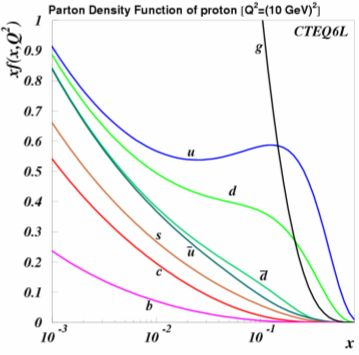
\includegraphics[width=.55\textwidth]{pdf}\hfill\parbox[b]{.44\textwidth}{
\caption{Parton distribution function obtained from the \textsc{cteq} collaboration. It gives the probability of extracting a specific quark from a proton with a certain fraction, $x$ of its energy. From \cite{scien2}.\label{pdff}}}
\end{figure}

The first complication would seem to be the lack of antiquarks in ordinary protons, however, as fig.~\ref{pdff} shows, at high energies there is a certain probability for extracting a wide variety of quarks from protons. These extra quarks are referred to as sea quarks. The functions that relate the probability of extracting a certain parton from a proton with the energy scale $Q^2$ and the momentum fraction of the extracted parton $x$ are called Parton Distribution Functions (PDFs)\footnote{PDFs may, if you like being confused, be classified as a type of probability density function (pdf).}, and are determined experimentally. This thesis will mainly deal with the CTEQ set of PDFs, but there are others.

This leads to the following equation, which relates the cross section of the interaction of interest, $\sigma(q\overline{q}\rightarrow\gamma\gamma)$ to the cross section of that process in proton-proton events, $\sigma(pp\rightarrow\gamma\gamma)$:
\(\sigma(pp\rightarrow\gamma\gamma)=\sum_q\iint dx_1\,dx_2\,f_q(x_1,Q^2)f_{\bar q}(x_2,Q^2)\sigma(q\bar q\rightarrow\gamma\gamma),\label{pdf}\)
where $f_q$ is the PDF for parton $q$.



\end{english}
\end{document}